\documentclass[a4paper,10pt]{book}
\usepackage{xeCJK}              
\usepackage[english]{babel}
\usepackage[utf8]{inputenc}
\usepackage[T1]{fontenc}
\usepackage{lmodern}
\usepackage{microtype}
\usepackage{natbib}
%% \usepackage{tocbibind}          
\usepackage{amsmath}
\usepackage{amsthm}
\usepackage[colorlinks=true,linkcolor=red]{hyperref}

\usepackage{color,xcolor}

\usepackage{indentfirst}
\setlength{\parindent}{2em}

\usepackage[onehalfspacing]{setspace}

\usepackage{hyperref}

\usepackage{pdfpages}
\usepackage{graphicx}

\usepackage{booktabs}
\usepackage{tcolorbox}

%% user defined command
\newcommand{\keyword}[1]{\textbf{#1}}
\newcommand{\lcmd}[1]{\texttt{#1}}
\newcommand{\head}[1]{\textnormal{\textbf{#1}}}
\usepackage{datetime}
\renewcommand{\today}{\number\year 年 \number\month 月 \number\day 日}

\usepackage{float}
\begin{document}

\begin{titlepage}
  \raggedleft
  {\Large 作者:\\\author[1in]}    
  {\large 此书关于\\}
  {\Huge\scshape \bookname\\[.2in]}      
  {\large \bookoneword\\}    
  \vfill
  {\itshape 首次编辑日期:\timeandcompany \\}
  {\itshape 最近编辑日期:\today}
\end{titlepage}

% Pages are numbered with lowercase Roman numbers.
% Chapters generate a table of contents entry but don't get a number.
\frontmatter

\tableofcontents{}
\listoffigures{}
\listoftables{}

% Pages are numbered with Arabic numbers.
% Chapters are numbered and produce a table of contents entry.
\mainmatter 


\chapter{\LaTeX\xspace Base}


\section{What is \LaTeX}
\label{sec:what-latex}

\LaTeX\index{latex} is a document markup language\footnote{Just like HTML}. It separate format from content.

\section{Reason to Use It}


Because \LaTeX \xspace{} is a markup language, you should learn it before you can use it.
So why should you spend so much time to learn it while there is so much document creator like Word, Pages?

There is several reasons that push me to select it.
\begin{itemize}
\item It provides powerful edit ability. You can almost get whatever you want to show, especially the mathematical equations.
\item Because it separate the format and the content, it is easy to do format alteration in the full document domain.
\item Once you create your own template, it is easy to wreate document with the template applied, saving so much time in format. 
\end{itemize}



\section{Logical formatting}
\index{latex!{logical formatting}}
\lstset{language=TeX}
\begin{lstlisting}
  \documentclass{article}
  \begin{document}
  \title{Example}
  \author{Mingming Li}
  \date{2022/11/04}
  \maketitle{}
  \section{Logical Formatting}
  This example show logical formatting.
  \end{document}
\end{lstlisting}

We do not specify the font family, font size, and so on, instead we tell \LaTeX \ the \keyword{class}, the \keyword{author}, or the \keyword{section} and let \LaTeX{} to format it.



\section{Command}
\index{latex!command}
LaTeX commands begin with a backslash, followed by big or small letters.
LaTeX commands are usually named with small letters and in a descriptive way.
There are exceptions: a backslash and just one special character.
Commands may have arguments, given in curly braces or in square brackets.

Calling a command looks like the following:


\begin{lstlisting}
  \command
  \command{argument}
  \command[optional argument]{argument}
\end{lstlisting}

For example

\begin{lstlisting}
  {\large Title}
  \usepackage{xeCJK}              
\usepackage[english]{babel}
\usepackage[utf8]{inputenc}
\usepackage[T1]{fontenc}
\usepackage{lmodern}
\usepackage{microtype}
\usepackage{natbib}
%% \usepackage{tocbibind}          
\usepackage{amsmath}
\usepackage{amsthm}
\usepackage[colorlinks=true,linkcolor=red]{hyperref}

\usepackage{color,xcolor}

\usepackage{indentfirst}
\setlength{\parindent}{2em}

\usepackage[onehalfspacing]{setspace}

\usepackage{hyperref}

\usepackage{pdfpages}
\usepackage{graphicx}

\usepackage{booktabs}
\usepackage{tcolorbox}

%% user defined command
\newcommand{\keyword}[1]{\textbf{#1}}
\newcommand{\lcmd}[1]{\texttt{#1}}
\newcommand{\head}[1]{\textnormal{\textbf{#1}}}
\usepackage{datetime}
\renewcommand{\today}{\number\year 年 \number\month 月 \number\day 日}

\usepackage{float}
  \documentclass[12pt]{article}
\end{lstlisting}

\section{Comment}
\index{latex!comment}
The percent sing(\%) introduces a \keyword{comment}.


\begin{lstlisting}
  \usepackage{xeCJK}              
\usepackage[english]{babel}
\usepackage[utf8]{inputenc}
\usepackage[T1]{fontenc}
\usepackage{lmodern}
\usepackage{microtype}
\usepackage{natbib}
%% \usepackage{tocbibind}          
\usepackage{amsmath}
\usepackage{amsthm}
\usepackage[colorlinks=true,linkcolor=red]{hyperref}

\usepackage{color,xcolor}

\usepackage{indentfirst}
\setlength{\parindent}{2em}

\usepackage[onehalfspacing]{setspace}

\usepackage{hyperref}

\usepackage{pdfpages}
\usepackage{graphicx}

\usepackage{booktabs}
\usepackage{tcolorbox}

%% user defined command
\newcommand{\keyword}[1]{\textbf{#1}}
\newcommand{\lcmd}[1]{\texttt{#1}}
\newcommand{\head}[1]{\textnormal{\textbf{#1}}}
\usepackage{datetime}
\renewcommand{\today}{\number\year 年 \number\month 月 \number\day 日}

\usepackage{float}  % include preamble tex file
\end{lstlisting}

\section{Environment}
\label{sec:environment}
\index{latex!environment}
\begin{lstlisting}
  % This is the environment syntax.
  \begin{name}[optional argument]{argument}
    ...
  \end{name}
\end{lstlisting}


\section{Breaks and Empty Lines}
\label{sec:breaks-empty-lines}

LaTeX treats multiple spaces just like a single space.
Also, a single line break has the same effect like a single space.
It doesn't matter how you arrange your text in the editor using spaces or breaks, the output will stay the same.
A blank line denotes a paragraph break.
Like spaces, multiple empty lines are treated as one.
Briefly said, spaces separate words, empty lines separate paragraphs.


\section{Special Symbols}
\label{sec:special-symbols}
\index{latex!symbols}
By putting a backslash before such a special symbol, we turned it into a LaTeX command.
This command has the only purpose of printing out that symbol.



\begin{lstlisting}
  \%  % just print % symbol
  \textbackslash % just print \ symbol
\end{lstlisting}




\section{Create Your Own Commands}

\begin{lstlisting}
  % This is the full definition of creating you own command.
  \newcommand{command}[arguments][optional]{definition}
\end{lstlisting}


\begin{lstlisting}
  % With no arguments.
  \newcommand{\TUG}{TeX Users Group\xspace}
  \TUG

  % With arguments.
  \newcommand{\keyword}[1]{\textbf{#1}}
  \keyword{declrations}

  % With optional arguments.
  \newcommand{\keyword2}[2][\bfseries]{{#1#2}}
  \keyword2[\itshape]{declarations}
\end{lstlisting}


\section{Get Help}
Three ways to get help about the package:
\begin{enumerate}
  
\item 
\begin{lstlisting}[language=sh]
    texdoc <package>
\end{lstlisting}

\item
\begin{lstlisting}[language=sh]
    kpsewhich <package>.sty
\end{lstlisting}

\item Visit the website: \url{http://ctan.org/pkg}

\end{enumerate}

\section{Install Extra Packages}
\label{sec:inst-extra-pack}

The easy way is to use the terminal to install extra packages:

\begin{lstlisting}[language=sh]
# Tex Live manager
tlmgr install <package>
\end{lstlisting}




\section{Floats}
\index{latex!float}


\LaTeX\xspace provides two floating environments, namely,
\argument{figure} and \argument{table}. They are briefly called
\keyword{floats}. Their content may float to a place where it's the
optimum for the page layout.


Here's the float placement options:
\begin{itemize}
\item h: here. The float may appear where it's been written in the source code.
\item t: top. Placing at the top of a page is permitted.
\item b: bottom. The float may appear at the bottom of a page.
\item p: page. The float is allowed to appear on a separate page,
  where only floats may reside but no normal text.
\item !: tells LaTeX to try harder! Some constraints may be ignored,
  easing the placement.
\end{itemize}


The most flexible is using the placement \argument{[!htbp]}, allowing a float
everywhere.







\section{Modes}
\label{sec:modes}

LaTeX knows three general \keyword{modes}:
\begin{itemize}
\item The \keyword{paragraph mode}: The text is typeset as a sequence of words in lines, paragraphs, and pages.
\item The \keyword{left-to-right mode}: The text is also considered to be a sequence of words, but LaTeX typesets it from left to right without breaking the line. 
\item The \keyword{math mode}: Letters are treated as math symbols. A lot of symbols can be used, most of them exclusively in this mode. Such symbols are roots, sum signs, relation signs, math accents, arrows, and various delimiters like brackets and braces. Space characters between letters and symbols are ignored. 
\end{itemize}



%%% Local Variables:
%%% mode: latex
%%% TeX-master: "latex"
%%% End:


\chapter{Emacs}
\label{cha:emacs}

Type all the \TeX\xspace commands is time consuming and error prone.
\keyword{Emacs} comes to the rescue. It can auto-fill the commands.

Emacs comes with a package for editing TeX and LaTeX files.
However, this package is extremely limited in its functionality.
A far better package called \keyword{AUC TeX} can help you write your papers efficiently.

Here is the Figure of using Emacs:
\begin{figure}[H]
  \centering
  \includegraphics[width=\textwidth]{emacs}
  \caption{Emacs}
  \label{fig:emacs}
\end{figure}


%%% Local Variables:
%%% mode: latex
%%% TeX-master: "latex"
%%% End:


\chapter[Commands and Environments]{Common Commands and Environments}

\section{Commands}
\label{sec:commands}


\lstset{language=TeX}
\begin{lstlisting}
% produces some space.
\quad                           

% ended a line.
\\ or \newline                  

% prevents a line break at the current position.
\nolinebreak                    

%  `` and '' is the quotation in latex. 
``hello''                       

% ragged left  
{\raggedleft Example text}      
% ragged right
{\raggedright Example text}     
% centering 
{\centering Example text}        


% tells LaTeX to produce a file with the extension .toc. 
% This file will be used to generate a table of contents. 
% We had to typeset twice: in the first run, the .toc file
% was written and in the second run, LaTeX read it and processed it.
\tableofcontents{}              


% causes a page break. Furthermore, the text has been 
% stretched to fill the page down to the bottom.
\pagebreak{}
% breaks the page as well, but it doesn't stretch the
% text: the remaining space of the page will stay empty.
\newpage{}
% forbids page breaking
\nopagebreak{}


% to squeeze more text onto a page. 
\enlargethispage{2\baselineskip}



% placed a superscripted number at the current position.
% Further, it prints its argument text into the bottom of 
% the page, marked by the same number
\footnote{text}
% modify the line that separates footnotes from the text 
% is produced by the command \footnoterule.
\renewcommand{\footnoterule}{\noindent\smash{\rule[3pt]{\textwidth}{0.4pt}}}

\rule[raising]{width}{height}
% draw a line 1pt at thick, as wide as text, raised a bit by 3 pt
\rule[3pt]{\textwidth}{1pt}

% \smash, we let our line pretend to have a height and a depth of 
zero, so it's occupying no vertical space at all


% when we use \footnote inside an argument, there will be an error. 
% \protect simply prevents this processing error. 
\protect{}
\section{Section \protect{\footnote{text}}}
% to avoid footnote appearing in heading and table of content
\section[title without footnote]{Section \protect{\footnote{text}}}



% ends the current page and causes all already defined figures and
tables to be printed out.
\clearpage{}

\cleardoublepage{}


% To be able to refer to a certain point, we have to mark it by a label.
% We can reference to the name of that label afterwards.
% notice , typeset twice to produce the cross reference
\label % marks the position
\ref % prints the number of the element we refer to 
\pageref % prints the page number of that element


\end{lstlisting}


\section{Environments}
\label{sec:environments}


\begin{lstlisting}
% quote long text
\begin{quotation}
\end{quotation}
\end{lstlisting}

\begin{lstlisting}
% center environment
\begin{center}
\end{center}
\end{lstlisting}


%%% Local Variables:
%%% mode: latex
%%% TeX-master: "latex"
%%% End:

\chapter{Font}

\section{Shape}
\begin{table}[!h]
  \centering
  \caption{Font Command}
  
  \begin{tabular}{ccc}
    \toprule
    \head{Command} & \head{Explaination} & \head{Output} \\
    \midrule
    \verb|\textbf{Example}| & bold font & \textbf{Example} \\
    \verb|\textit{Example}| & italic & \textit{Example} \\
    \verb|\textsl{Example}| & slated & \textsl{Example} \\
    \verb|\textsc{Example}| & small caps & \textsc{Example} \\
    \verb|\textup{Example}| & & \textup{Example} \\
    \verb|\textmd{Example}| & medium & \textmd{Example} \\
    \verb|\textnormal{Example}| & & \textnormal{Example} \\
    \verb|\textsf{Example}| & sans-serif & \textsf{Example} \\
    \verb|\texttt{Example}| & typewritter & \texttt{Example} \\
    \verb|\textrm{Example}| & Roman & \textrm{Example} \\
    \bottomrule
    
  \end{tabular}
  
\end{table}


\begin{table}[!h]
  \centering
  \caption{Font Declaration}
  \begin{tabular}{ccc}
    \toprule
    \head{Declaration} & \head{Explaination} & \head{Output} \\
    \midrule
    \verb|{\itshape Example}| & italic & {\itshape Example} \\
    \verb|{\bfseries Example}| & bold font & {\bfseries Example} \\
    \verb|{\slshape Example}| & slated & {\slshape Example} \\
    \verb|{\scshape Example}| & small caps & {\scshape Example} \\
    \verb|{\upshape Example}| & & {\upshape Example} \\
    \verb|{\mdseries Example}| & medium & {\mdseries Example} \\
    \verb|{\normalfont Example}| & & {\normalfont Example} \\
    \verb|{\sffamily Example}| & sans-serif & {\sffamily Example} \\
    \verb|{\ttfamily Example}| & typewritter & {\ttfamily Example} \\
    \verb|{\rmfamily Example}| & roman & {\rmfamily Example} \\
    \bottomrule
    
  \end{tabular}
  
\end{table}


\begin{table}[!hbp]
  \centering
  \caption{Font Emphasized}
  \begin{tabular}{ccc}
    \toprule
    \head{Command} & \head{Explaination} & \head{Output} \\
    \midrule
    \verb|\emph{Example}| & emphasized & \emph{Example} \\
    \bottomrule
  \end{tabular}
\end{table}
\clearpage



\section{Size}
\begin{table}[!hbp]
  \centering
  \caption{Font Size}
  \begin{tabular}{cc}
    \toprule
    \head{Command} & \head{Output} \\
    \midrule
    \verb|\tiny{Example}| & \tiny{Example} \\
    \verb|\scriptsize{Example}| & \scriptsize{Example} \\
    \verb|\footnotesize{Example}| & \footnotesize{Example} \\
    \verb|\small{Example}| & \small{Example} \\
    \verb|\normalsize{Example}| & \normalsize{Example} \\
    \verb|\large{Example}| & \large{Example} \\
    \verb|\Large{Example}| & \Large{Example} \\
    \verb|\LARGE{Example}| & \LARGE{Example} \\
    \verb|\huge{Example}| & \huge{Example} \\
    \verb|\Huge{Example}| & \Huge{Example} \\
    \bottomrule
  \end{tabular}
\end{table}



\chapter{Box}

\section{parbox}

We used the command \lstinline{\parbox} to create a column.

\begin{lstlisting}
  \parbox[alignment]{width}{text}
  \parbox[alignment][height][inner alignment]{width}{text}
\end{lstlisting}

\begin{description}
\item[alignment] Optional argument for the vertical alignment. State t to align at the top line of the box; write b to align at its bottom line. The default behavior is to place the box such that its center is in line with the center of the current text line.
\item[height] If this optional argument isn't given, the box will have just the natural height of the text inside. Use this argument if you want to change the height of the box to make it bigger or smaller.
\item[inner alignment] Especially, if the height of the box is different to the natural height of the contained text, you might want to adjust the text position. The argument means:
  \begin{itemize}
  \item c: vertically center the text in the box
  \item t: place text at the top of the box
  \item b: place text at its bottom
  \item s: stretch the text vertically if possible
  \end{itemize}
  
\end{description}

\begin{lstlisting}
Text line
\quad\fbox{\parbox[b]{1.8cm}{this parbox is aligned at its bottom line}}
\quad\fbox{\parbox{1.5cm}{center-aligned parbox}}
\quad\fbox{\parbox[t]{2cm}{another parbox aligned at its top line}}
\end{lstlisting}


Text line
\quad\fbox{\parbox[b]{1.8cm}{this parbox is aligned at its bottom line}}
\quad\fbox{\parbox{1.5cm}{center-aligned parbox}}
\quad\fbox{\parbox[t]{2cm}{another parbox aligned at its top line}}


\section{fbox}

This command show the frame out.

\begin{lstlisting}
  \fbox{Example}
\end{lstlisting}

\fbox{Example}


\section{minipage}
\label{sec:minipage}

Parboxes are suitable for boxes with only a little text inside.
In case of a box containing a large amount of text, the closing brace could easily be forgotten or overlooked.
The minipage environment would then be a better choice.


\begin{lstlisting}
  \begin{minipage}{3cm}
    Hello World!
  \end{minipage}
\end{lstlisting}

\begin{minipage}{3cm}
  Hello World!
\end{minipage}

\section{mbox}
\label{sec:mbox}


\begin{lstlisting}
  \mbox{Hello World}
\end{lstlisting}

\mbox{Hello World}

\section{tcolorbox}
\label{sec:tcolorbox}

\begin{lstlisting}
\begin{tcolorbox}
  \mbox{Hello World}
\end{tcolorbox}
\end{lstlisting}

\begin{tcolorbox}
  \mbox{Hello World}
\end{tcolorbox}


\chapter{Lists}
\label{cha:lists}


\section{Bulleted Lists}

\begin{lstlisting}
  \begin{itemize}
  \item geometry
  \item amsmath
  \end{itemize}
\end{lstlisting}


\begin{itemize}
\item geometry
\item amsmath
\end{itemize}


\section{Numbered Lists}
\begin{lstlisting}
  \begin{enumerate}
  \item geometry
  \item amsmath
  \end{enumerate}
\end{lstlisting}


\begin{enumerate}
\item geometry
\item amsmath
\end{enumerate}




\section{Definition Lists}
\begin{lstlisting}
  \begin{description}
  \item[paralist] provides compact lists and list versions that
    can be used within paragraphs, helps to customize labels and
    layout
  \item[enumitem] gives control over labels and lengths
    in all kind of lists
  \item[mdwlist] is useful to customize description lists, it
    even allows multi-line labels. It features compact lists and
    the capability to suspend and resume.
  \item[desclist] offers more flexibility in definition list
  \item[multenum] produces vertical enumeration in multiple
    columns
  \end{description}
\end{lstlisting}


\begin{description}
\item[paralist] provides compact lists and list versions that
  can be used within paragraphs, helps to customize labels and
  layout
\item[enumitem] gives control over labels and lengths
  in all kind of lists
\item[mdwlist] is useful to customize description lists, it
  even allows multi-line labels. It features compact lists and
  the capability to suspend and resume.
\item[desclist] offers more flexibility in definition list
\item[multenum] produces vertical enumeration in multiple
  columns
\end{description}


%%% Local Variables:
%%% mode: latex
%%% TeX-master: "latex"
%%% End:

\documentclass{article}
\begin{document}

\newcommand{\head}[1]{\textnormal{\textbf{#1}}}

\begin{tabular}{c|c@{\{example\}*3}c}
  \hline                      % Draw a horizontal line over whole width of the table
  \head{Command} & \head{Declaration} & \head{Output} \\
  \hline
  \verb|\textrm| & \verb|\rmfamily| & \rmfamily Example text \\
  \verb|\textsf| & \verb|\sffamily| & \sffamily Example text \\
  \verb|\texttt| & \verb|\ttfamily| & \ttfamily Example text \\
  \hline
\end{tabular}

\end{document}
%%% Local Variables:
%%% mode: latex
%%% TeX-master: t
%%% End:

\chapter{Figure}

\argument{graphicx} is need to insert figure into you document.


LaTeX supports the following file types:
\begin{itemize}
\item \argument{PNG, JPG}, and \argument{PDF} if you directly compile
  to PDF (\keyword{pdfLaTeX})
\item \argument{EPS} if you compile to DVI and convert to PS and PDF (traditional LaTeX)
\end{itemize}


\begin{tcolorbox}
  \begin{itemize}
  \item PS: PostScript
  \item EPS: Encapsulated PostScript
  \item DVI: Device Independent Format
  \end{itemize}
\end{tcolorbox}


You don't need to specify a filename extension, it will be
automatically added.
Don't use blanks in the filename or path!
Blanks and special characters may cause problems with \lstinline|\includegraphics|.
If such symbols in filenames are required, load the package
\argument{grffile} to try to fix it.


\begin{lstlisting}
  \usepackage[demo]{graphicx}
  \begin{figure}
    \centering
    \includegraphics{test}
    \caption{Test figure}
  \end{figure}
\end{lstlisting}

Because we specified the \argument{demo} option, \argument{graphicx}
doesn't require a file \argument{test.png} or any other file; instead
it's just printing a black filled rectangle. This is useful for
testing or if you would like to discuss a LaTeX problem in an online
forum, but don't wish to publish your pictures.


\begin{lstlisting}
  % syntax
  \includegraphics[k=v]{file name}
\end{lstlisting}

Here are the most popular ones:
\begin{itemize}
\item \argument{width}: \lstinline|width=0.8\textwidth|
\item \argument{height}
\item \argument{scale}: \lstinline|scale=0.5|
\item \argument{angle}: \lstinline{angle=90}
\end{itemize}







\chapter{Listing Content and References}
\label{cha:list-cont-refer}



\section{Table of Content}
\label{sec:table-content}

\begin{table}[H]
  \centering
  \begin{tabular}{>{\textbackslash\ttfamily}ll}
    \toprule
    \normal{\head{Command}} & \head{Level}\\
    \midrule
    part & -1 (\argument{book} and \argument{report} class)\\
    chapter & 0 (not available in \argument{article})\\
    section & 1\\
    subsection & 2\\
    subsubsection & 3\\
    paragraph & 4\\
    subparagraph & 5\\
    \bottomrule
  \end{tabular}
  \caption{Depth of the TOC}
  \label{tab:depth-of-toc}
\end{table}


There's a variable representing the level, namely, \lstinline|\tocdepth|.
It's an integer variable which we call a \keyword{counter}.

There are two basic ways to adjust a counter value:
\begin{lstlisting}
% specifies an integer value of 'n' for the counter 'name'.
\setcounter{name}{n}            
% adds the integer value of 'n' to value of the counter 'name'. 'n' may be negative.
\addtocounter{name}{n}          


\setcounter{tocdepth}{3}
% you can raise or lower the level without knowing its number.
\addtocounter{tocdepth}{1}
\end{lstlisting}


\subsection{Adding entries manually}
\label{sec:adding-entr-manu}

\begin{lstlisting}
% file extension:
% toc: table of contents file
% lof: list of figures file
% lot: list of tables file

% sectional unit: part, chapter, section, subsection, paragraph, subparagraph
\addcontentsline{file extension}{sectional unit}{text}

% In contrary to \addcontentsline, the argument entry is written directly to the file
% without any additional formatting. You may choose any formatting you like.
\addtocontents{file extension}{entry}


% Examples
\addcontentsline{toc}{chapter}{Preface}
\addcontentsline{toc}{part}{Appendix}

\addtocontents{toc}{\bigskip}
% extends the text height such that one additional line fits to the contents page.
\addtocontents{toc}{\protect\enlargethispage{\baselineskip}}
% causes a page break in the TOC.
\addtocontents{toc}{\protect\newpage} 
% changes the page style of the current TOC page to fancy.
\addtocontents{toc}{\protect\thispagestyle{fancy}} 

\end{lstlisting}



\section{Creating and Customizing Lists of Figures}
\label{sec:creat-cust-lists}

\begin{lstlisting}
% renamed the figures and the list heading 
\renewcommand{\figurename}{Diagram}
\renewcommand{\listfigurename}{List of Diagrams}
\listoffigures
\end{lstlisting}


\section{Creating and Customizing Lists of Tables}
\label{sec:creat-cust-lists-1}

\begin{lstlisting}
\renewcommand{\tablename}{Diagram}
\renewcommand{\listtablename}{List of Diagrams}
\listoffigures
\end{lstlisting}


\section{Generating an Index}
\label{sec:generating-an-index}

Steps to generating index list:
\begin{enumerate}
\item load the index package and add the command to create the index
\begin{lstlisting}
\usepackage{index}
\makeindex{}
\end{lstlisting}

\item mark index point
\begin{lstlisting}
% simple entry
\index{entry}
% example \index{enterprise}                   

% subentry
\index{entry!subentry}          
% example \index{enterprise!organization}

% subsubentry
\index{entry!subentry!subsubentry} 
% example \index{enterprise!organization!operation}

This will be written to a file with the extension .idx.
\end{lstlisting}

\item create an entry for the index for the table of contents
\begin{lstlisting}
\clearpage
\addcontentsline{toc}{chapter}{Index}
\end{lstlisting}

\item in the next line, typeset the index
\begin{lstlisting}
\printindex{}
\end{lstlisting}

\item use shell command to typeset the tex document \label{item:1}
\begin{lstlisting}[language=sh]
xelatex latex.tex               # .tex is optional
# or
pdflatex latex.tex              # .tex is optional
\end{lstlisting}
  
\item use shell command to produce \argument{.idx} file.
\begin{lstlisting}[language=sh]
makeindex latex.idx             # .idx is optional
\end{lstlisting}
  
\item typeset the tex document again, refer to \ref{item:1}
  
\end{enumerate}


\subsection{Specifying Page Ranges}
\label{sec:spec-page-rang}

\begin{lstlisting}
% Example
\index{network|(}
...
\index{network|)}
\end{lstlisting}


\subsection[Symbols in the Index]{Using Symbols in the Index}
\label{sec:using-symbols-macros}

\argument{makeindex} sorts the entries alphabetically.
If you would like to include symbols in the index, for example, Greek letters, chemical formulas, or math symbols, you could face the problem of integrating them into the sorting.
For this purpose, \lstinline|\index| understands a sort key.
Use this key as prefix for the entry, separated by an @ symbol, for instance:
\begin{lstlisting}
\index{Gamma@$\Gamma$}
\end{lstlisting}

\subsection{Referring to Other Index Entries}
\label{sec:referr-other-index}


Different words may stand for the same concept.
For such cases, it's possible to add a cross-reference to the main phrase without a page number.
Adding the code \lstinline.see{entry list}. achieves that, for example:
\begin{lstlisting}
\index{network|see{WLAN}}
\index{WLAN}
\end{lstlisting}

As such references don't print a page number, their position in the text doesn't matter. You could collect them in one place of your document.


\subsection{Fine-tuning Page Numbers}
\label{sec:fine-tuning-page}

If an index entry refers to several pages, you might want to emphasize one page number to indicate it as the primary reference.
You could define a command for emphasizing as follows:
\begin{lstlisting}
\newcommand{\main}[1]{\emph{#1}}
\index{WLAN|main}
\end{lstlisting}


\subsection{Designing the Index Layout}
\label{sec:design-index-layo}

LaTeX provides some index styles called \keyword{latex} (the default), \keyword{gind, din}, and \keyword{iso}.
To use another style, specify it using the \argument{–s} option of the makeindex program, for example:
\begin{lstlisting}[language=sh]
makeindex -s iso latex
\end{lstlisting}


\section{Creating a Bibliography}
\label{sec:creat-bibl}

\begin{lstlisting}
\begin{thebibliography}{widest label}
   \bibitem[label]{key} author, title, year etc.
   \bibitem...
   ...
\end{thebibliography}
\end{lstlisting}


\begin{lstlisting}
% Example
To study \TeX\ in depth, see \cite{DK86}. 
For writing math texts, see \cite{DK89}.


\begin{thebibliography}{8}
\bibitem{DK86} D.E. Knuth, \emph{The {\TeX}book}, 1986
\bibitem{DK89} D.E. Knuth, \emph{Typesetting Concrete Mathematics}, 1989
\end{thebibliography}
\end{lstlisting}

Each item is specified using the command \lstinline|\bibitem|.
This command requires a mandatory argument determining the \argument{key}.
We may simply refer to this key by \lstinline|\cite{key}| or \lstinline|\cite{key1,key2}|.
\lstinline|\cite| accepts an optional argument stating a page range, for example, \lstinline|\cite[p.\,18--20]{key}|.
You may choose a label by the optional argument of \lstinline|\bibitem|.
If no label has been given, LaTeX will number the items consecutively in square brackets.


\subsection[Bibtex]{Using Bibliography Databases With Bibtex}
\label{sec:using-bibl-datab}


\begin{enumerate}
\item Create a new document. For example \argument{latex.bib}.
\begin{lstlisting}
@book{DK86,
author = "D.E. Knuth",
title = "The {\TeX}book",
publisher = "Addison Wesley",
year = 1986
}

@article{DK89,
author = "D.E. Knuth",
title = "Typesetting Concrete Mathematics",
journal = "TUGboat",
volume = 10,
number = 1,
pages = "31--36",
month = apr,
year = 1989
}
\end{lstlisting}

\item Include the database in to your tex document. For example \argument{latex.tex}.
\begin{lstlisting}
\bibliographystyle{alpha}       % plain, unsrt, alpha, abbrv
\bibliography{latex}            % latex stands for latex.bib here
\end{lstlisting}
  
\item Typeset one time with \keyword{pdfLaTeX} or \keyword{xelatex}.
\begin{lstlisting}
xelatex latex
\end{lstlisting}
  
\item \argument{bibtex} document.
\begin{lstlisting}[language=sh]
bibtex latex                    # here latex is the documentname
\end{lstlisting}
  
\item Typeset again the tex file.
\end{enumerate}

\section{Changing the Headings}
\label{sec:changing-headings}

You can use \lstinline|\renewcommand| to change the headings.


\begin{table}[H]
  \centering
  \begin{tabular}{l>{\textbackslash\ttfamily}ll}
    \toprule
    \head{List} & \normal{\head{Heading Command}} & \head{Default heading}\\
    \midrule
    Table of contents & contentsname & \keyword{Contents}\\
    List of figures & listfigurename & \keyword{List of figures}\\
    List of tables & listtablename & \keyword{List of tables}\\
    \multirow{2}{*}{Bibliography} & bibname in book and report & \keyword{Bibliography} in book and report\\
                & refname in article & \keyword{References} in article\\
    Index & indexname & \keyword{index}\\
    \bottomrule
  \end{tabular}
  \caption{Headings name}
  \label{tab:headings}
\end{table}

\begin{table}[H]
  \centering
  \begin{tabular}{l>{\textbackslash\ttfamily}l>{\bfseries}l}
    \toprule
    \head{Name} & \normal{\head{Heading Command}} & \head{Default heading}\\
    \midrule
    figure & figurename & Figure\\
    table & tablename & Table\\
    part & partname & Part\\
    chapter & chaptername & Chapter\\
    abstract & abstractname & Abstract\\
    appendix & appendixname & Appendix\\
    \bottomrule

  \end{tabular}
  \caption{Macros name}
  \label{tab:macros-name}
\end{table}


%%% Local Variables:
%%% mode: latex
%%% TeX-master: "latex"
%%% End:


\chapter{Math}
\label{cha:probability}

\section{Markov chain}
\label{sec:markov-chain}

A \keyword{Markov chain} or \keyword{Markov process} is a stochastic model describing a sequence of possible events in which the probability of each event depends only on the state attained in the previous event.

\subsection{Transitions}
\label{sec:transitions}

The changes of state of the system are called \keyword{transitions}.
The probabilities associated with various state changes are called \keyword{transition probabilities}.
The process is characterized by a state space, a transition matrix describing the probabilities of particular transitions, and an initial state (or initial distribution) across the state space.

\subsection{Discrete-time Markov chain}
\label{sec:discrete-time-markov}

A \keyword{discrete-time Markov chain} is a sequence of random variables $X_1, X_2, X_3, \ldots$ with the Markov property, namely that the probability of moving to the next state depends only on the present state and not on the previous states:
\begin{equation}
  \label{eq:14}
   \operatorname{P}\left(X_{n+1}=x \mid X_1=x_1, X_2=x_2, \ldots, X_n=x_n\right)=\operatorname{P}\left(X_{n+1}=x \mid X_n=x_n\right)
\end{equation}

if both conditional probabilities are well defined, that is, if \(\operatorname{P}\left(X_1=x_1, \ldots, X_n=x_n\right)>0\).



The possible values of $X_i$ form a countable set $S$ called the state space of the chain.


\subsection{Continous-time Markov chain}
\label{sec:cont-time-mark}

A \keyword{continuous-time Markov chain} $\mathrm{X}(\mathrm{t})$ is defined by two components: a jump chain, and a set of holding time parameters $\lambda_i$.
The jump chain consists of a countable set of states $\mathrm{S} \subset\{0,1,2, \cdots\}$ along with transition probabilities $\mathrm{p}_{\mathrm{ij}}$.
We assume $\mathrm{p}_{\mathrm{ii}}=0$, for all non-absorbing states $\mathrm{i} \in \mathrm{S}$.
We assume
\begin{enumerate}
\item if $X(t)=i$, the time until the state changes has Exponential $\left(\lambda_{\mathrm{i}}\right)$ distribution;
\item if $X(t)=i$, the next state will be $j$ with probability $p_{i j}$.
\end{enumerate}

The process satisfies the Markov property.
That is, for all $0 \leq \mathrm{t}_1<\mathrm{t}_2<\cdots<\mathrm{t}_{\mathrm{n}}<\mathrm{t}_{\mathrm{n}+1}$, we have
$$
\begin{aligned}
\mathrm{P}\left(\mathrm{X}\left(\mathrm{t}_{\mathrm{n}+1}\right)=\mathrm{j} \mid \mathrm{X}\left(\mathrm{t}_{\mathrm{n}}\right)\right. & \left.=\mathrm{i}, \mathbf{X}\left(\mathrm{t}_{\mathrm{n}-1}\right)=\mathrm{i}_{\mathrm{n}-1}, \cdots, X\left(\mathrm{t}_1\right)=\mathrm{i}_1\right) \\
& =\mathrm{P}\left(\mathrm{X}\left(\mathrm{t}_{\mathrm{n}+1}\right)=\mathrm{j} \mid \mathbf{X}\left(\mathrm{t}_{\mathrm{n}}\right)=\mathrm{i}\right)
\end{aligned}
$$


\subsection{Markov kernel}
\label{sec:markov-kernel}


Let $(X, \mathcal{A})$ and $(Y, \mathcal{B})$ be \keyword{measurable spaces}.
A \keyword{Markov kernel} with source $(X, \mathcal{A})$ and target $(Y, \mathcal{B})$ is a map $\kappa: \mathcal{B} \times X \rightarrow[0,1]$ with the following properties:
\begin{enumerate}
\item For every (fixed) $B \in \mathcal{B}$, the map $x \mapsto \kappa(B, x)$ is $\mathcal{A}$-measurable
\item For every (fixed) $x \in X$, the map $B \mapsto \kappa(B, x)$ is a \keyword{probability measure} on $(Y, \mathcal{B})$
\end{enumerate}

In other words it associates to each point $x \in X$ a probability measure $\kappa(d y \mid x): B \mapsto \kappa(B, x)$ on $(Y, \mathcal{B})$ such that, for every measurable set $B \in \mathcal{B}$, the map $x \mapsto \kappa(B, x)$ is measurable with respect to the $\sigma$-algebra $\mathcal{A}$.


\subsection{Measurable space}
\label{sec:measurable-space}

A \keyword{measurable space} consists of a set and a \keyword{\(\sigma\)-algebra}, which defines the subsets that will be measured.

Consider a set \(X\) and a \(\sigma\)-algebra \(\mathcal{A}\) on \(X\).
Then the tuple \((X, \mathcal{A})\) is called a measurable space.

\subsection{\protect{\(\sigma\)}-algebra}


A \keyword{\(\sigma\)-algebra} (also \(\sigma\)-field) on a set \(X\) is a nonempty collection \(\Sigma\) of subsets of \(X\) closed under complement, countable unions, and countable intersections.

Let $X$ be some set, and let $P(X)$ represent its power set.
Then a subset $\Sigma \subseteq P(X)$ is called a $\sigma$-algebra if it satisfies the following three properties:
\begin{enumerate}
\item $X$ is in $\Sigma$, and $X$ is considered to be the universal set in the following context.
\item $\Sigma$ is closed under complementation: If $A$ is in $\Sigma$, then so is its complement, $X \backslash A$.
\item $\Sigma$ is closed under countable unions: If $A_1, A_2, A_3, \ldots$ are in $\Sigma$, then so is $A=A_1 \cup A_2 \cup A_3 \cup \cdots$.
\end{enumerate}

From these properties, it follows that the $\sigma$-algebra is also closed under countable intersections (by applying De Morgan's laws).

\section{Conditional probability}
\label{sec:cond-prob}

Given two events \(A\) and \(B\).

\begin{equation}
  \label{eq:19}
  P(A \mid B)=\frac{P(A \cap B)}{P(B)}
\end{equation}

\(P(A|B)\) stands for the probability of A happening given that B happened.
\(P(A \cap B)\) stands for the probability of A and B happening at the same time.
\(P(B)\) stands for the probability of B happening.
\section{Posterior probability}
\label{sec:post-prob}

The \keyword{posterior probability} is a type of conditional probability that results from updating the prior probability with information summarized by the likelihood via an application of Bayes' rule.

In variational Bayesian methods, the posterior probability is the probability of the parameters $\theta$ given the evidence $X$, and is denoted $p(\theta \mid X)$.
It contrasts with the likelihood function, which is the probability of the evidence given the parameters: $p(X \mid \theta)$.

The two are related as follows:
Given a prior belief that a probability distribution function is $p(\theta)$ and that the observations $x$ have a likelihood $p(x \mid \theta)$, then the posterior probability is defined as

\begin{equation}
  \label{eq:20}
  p(\theta \mid x)=\frac{p(x \mid \theta)}{p(x)} p(\theta)  
\end{equation}

where $p(x)$ is the normalizing constant and is calculated as
\begin{equation}
  \label{eq:21}
  p(x)=\int p(x \mid \theta) p(\theta) d \theta  
\end{equation}




\section{Guassian distribution}
\label{sec:guass-distr}


\keyword{Gaussian distribution} (normal distribution) is a type of continuous probability distribution for a real-valued random variable.
The general form of its probability density function is
\begin{equation}
  \label{eq:22}
  f(x)=\frac{1}{\sigma \sqrt{2 \pi}} e^{-\frac{1}{2}\left(\frac{x-\mu}{\sigma}\right)^2}  
\end{equation}


The parameter $\mu$ is the mean or expectation of the distribution (and also its median and mode), while the parameter $\sigma$ is its standard deviation.
The variance of the distribution is $\sigma^2$.
The Figure \ref{fig:gaussian-distribution} shows the Gaussian distributions.

\begin{figure}[!htp]
  \centering
  \includegraphics[width=0.8\textwidth]{images/gaussian-distribution}
  \caption{Gaussian distribution}
  \label{fig:gaussian-distribution}
\end{figure}
\section{Laplace distribution}
\label{sec:laplace-distribution}

A random variable has a Laplace $(\mu, b)$ distribution if its probability density function is
\begin{equation}
  \label{eq:23}
  f(x)=\frac{1}{2 b} \exp \left(-\frac{|x-\mu|}{b}\right)  
\end{equation}

Here \(\mu\) is a location parameter and \(b\) is a scale parameter.
Figure \ref{fig:laplace-distribution} shows the Laplace distributions.

\begin{figure}[!htp]
  \centering
  \includegraphics[width=0.8\textwidth]{images/laplace-distribution}
  \caption{Laplace distribution}
  \label{fig:laplace-distribution}
\end{figure}

\section{Monte Carlo method}
\label{sec:monte-carlo-method}

\keyword{Monte Carlo methods} are a broad class of computational algorithms that rely on repeated random sampling to obtain numerical results.
The underlying concept is to use randomness to solve problems that might be deterministic in principle.


Monte Carlo methods vary, but tend to follow a particular pattern:
\begin{enumerate}
\item Define a domain of possible inputs
\item Generate inputs randomly from a probability distribution over the domain
\item Perform a deterministic computation on the inputs
\item Aggregate the results
\end{enumerate}



\section{Variational Bayesian methods}
\label{sec:vari-bayes-meth}


It is a simplifying that makes the intractable events into tractable events.

For example,
in variational inference, the posterior distribution over a set of unobserved variables $\mathbf{Z}=\left\{Z_1 \ldots Z_n\right\}$ given some data $\mathbf{X}$ is approximated by a so-called variational distribution, $Q(\mathbf{Z})$:
\begin{equation}
  \label{eq:26}
  P(\mathbf{Z} \mid \mathbf{X}) \approx Q(\mathbf{Z})  
\end{equation}


The distribution $Q(\mathbf{Z})$ is restricted to belong to a family of distributions of simpler form than $P(\mathbf{Z} \mid \mathbf{X})$ (e.g. a family of Gaussian distributions), selected with the intention of making $Q(\mathbf{Z})$ similar to the true posterior, $P(\mathbf{Z} \mid \mathbf{X})$.

The similarity (or dissimilarity) is measured in terms of a dissimilarity function $d(Q ; P)$ and hence inference is performed by selecting the distribution $Q(\mathbf{Z})$ that minimizes $d(Q ; P)$.
The most common type of variational Bayes uses the Kullback-Leibler divergence (KL-divergence) of $Q$ from $P$ as the choice of dissimilarity function. 

\section{Bayesian probability}
\label{sec:bayesian-probability}

Bayesian probability is an interpretation of the concept of probability, in which, instead of frequency or propensity of some phenomenon, probability is interpreted as reasonable expectation representing a state of knowledge or as quantification of a personal belief.

\section{Binomial distribution}
\label{sec:binom-distr}

In general, if the random variable $X$ follows the binomial distribution with parameters $n \in \mathbb{N}$ and $p \in$ $[0,1]$, we write $X \sim \mathrm{B}(n, p)$.
The probability of getting exactly $k$ successes in $n$ independent Bernoulli trials is given by the probability mass function:
\begin{equation}
  \label{eq:24}
  f(k)=\left(\begin{array}{l}
               n \\
               k
             \end{array}\right) p^k(1-p)^{n-k}
\end{equation}

for $k=0,1,2, \ldots, n$, where
\begin{equation}
  \label{eq:25}
\left(\begin{array}{l}
n \\
k
\end{array}\right)=\frac{n !}{k !(n-k) !}
\end{equation}

The figure \ref{fig:binomial-distribution} shows the distribution.
\begin{figure}[!htp]
  \centering
  \includegraphics[width=0.6\textwidth]{images/binomian-distribution.png}
  \caption{Binomial distribution}
  \label{fig:binomial-distribution}
\end{figure}

\section{Kullback–Leibler divergence}
\label{sec:kullb-diverg}


The Kullback-Leibler divergence, denoted $D_{\mathrm{KL}}(P \| Q)$, is a type of statistical distance: a measure of how one probability distribution $P$ is different from a second, reference probability distribution $Q$.


For discrete probability distributions $P$ and $Q$ defined on the same sample space, $\mathcal{X}$, the relative entropy from $Q$ to $P$ is defined ${ }^{[11]}$ to be
\begin{equation}
  \label{eq:27}
  D_{\mathrm{KL}}(P \| Q)=\sum_{x \in \mathcal{X}} P(x) \log \left(\frac{P(x)}{Q(x)}\right) .  
\end{equation}


which is equivalent to
\begin{equation}
  \label{eq:28}
  D_{\mathrm{KL}}(P \| Q)=-\sum_{x \in \mathcal{X}} P(x) \log \left(\frac{Q(x)}{P(x)}\right)  
\end{equation}

\section{Jensen's inequality}
\label{sec:jensens-inequality}

Jensen's inequality generalizes the statement that a secant line of a convex function lies above its graph.

Thus, Jensen's inequality is
\begin{equation}
  \label{eq:40}
f\left(t x_1+(1-t) x_2\right) \leq t f\left(x_1\right)+(1-t) f\left(x_2\right) .  
\end{equation}

Shown in Figure \ref{fig:jenson-equality}.

\begin{figure}[!htp]
  \centering
  \includegraphics[width=0.6\textwidth]{images/jensen-inequality.png}
  \caption{Jensen's inequality}
  \label{fig:jenson-equality}
\end{figure}


In the context of probability theory, it is generally stated in the following form: if $X$ is a random variable and $\varphi$ is a convex function, then
\begin{equation}
  \label{eq:41}
\varphi(\mathrm{E}[X]) \leq \mathrm{E}[\varphi(X)]  
\end{equation}

The difference between the two sides of the inequality, $\mathrm{E}[\varphi(X)]-\varphi(\mathrm{E}[X])$, is called the Jensen gap.



%%% Local Variables:
%%% mode: latex
%%% TeX-master: "machine-learning"
%%% End:


\chapter{Using Fonts}
\label{cha:using-fonts}

\section{Installing Additional Fonts}
\label{sec:inst-addit-fonts}

TeX distributions usually install a lot of fonts.
A package manager allows the installation of further fonts, like mpm with MiKTeX or tlmgr with TeX Live.



TeX Live includes only freely licensed fonts.
Non-free fonts may be installed using a separate program. It's called getnonfreefonts. 

\begin{lstlisting}[language=Sh]
# Install getnonfreefonts
wget https://www.tug.org/fonts/getnonfreefonts/install-getnonfreefonts
texlua install-getnonfreefonts
\end{lstlisting}


Using the following commands to get the usage of commands:
\begin{lstlisting}[language=Sh]
getnonfreefonts --user -h  
getnonfreefonts --sys -h  
\end{lstlisting}


\section{Choosing the Main Font}
\label{sec:choosing-main-font}

\begin{lstlisting}
\usepackage{lmodern}
\end{lstlisting}





%%% Local Variables:
%%% mode: latex
%%% TeX-master: "latex"
%%% End:


\chapter{Developing Large Documents}
\label{cha:devel-large-docum}


\section{Spliting the Input}
\label{sec:spliting-input}


Using ``divide and conquer'' thought to develop large documents, i.e. break down a document into several sub-documents.

There are two common commands to combine the sub-documents into a large document:
\begin{lstlisting}
\input{filename}
\include{filename}
\end{lstlisting}

When LaTeX encounters \lstinline|\input| command, it reads in the file with the name \argument{filename} exactly as if its contents have been typed at that point.
Accordingly, all commands in this file would be processed by the LaTeX compiler.
You can even nest \lstinline|\input| — this command may be used inside an included file.

The argument is treated the same way as \lstinline|\input|.
However, there are some important differences:
\begin{enumerate}
\item \lstinline|\include| implicitly starts new pages. \lstinline|\include{filename}| behaves like:
\begin{lstlisting}
\clearpage
\include{filename}
\clearpage
\end{lstlisting}
  
\item \lstinline|\include| cannot be nested.

\item \lstinline|\include| supports a mechanism of choosing which parts of the document you wish to compile (\lstinline|\includeonly|).
\end{enumerate}


\begin{lstlisting}
\includeonly{file list}
\end{lstlisting}

The argument may be a comma-separated list of filenames.
If a file, \argument{name.tex}, is not specified within this argument, \lstinline|\include{name}| would not insert this file but just behave like \clearpage instead.
This allows excluding chunks or whole chapters from compiling.
If you work on a huge document, this speeds up compilation if you choose to include just your current chapter while keeping the labels and references of the excluded chapter this way.

\section{Creating Front and Back Matter}
\label{sec:creating-front-back}

Books often begin with introductory material such as copyright information, a foreword, acknowledgements, or a dedication. This part, including the title page and the table of contents, is called the \keyword{front matter}.
At the end, a book might include an afterword and supporting material like a bibliography, and an index. This part is called the \keyword{back matter}.


\begin{lstlisting}
\documentclass{article}
\begin{document}

% Pages are numbered with lowercase Roman numbers.
% Chapters generate a table of contents entry but don't get a number.
\frontmatter 
\chapter*{Dedication}

我学习项目管理的目的有三个:
\begin{itemize}
\item 考取PMP证书。
\item 开阔自己的视野,从更广的角度去思考问题。
\item 指导自己的生活,将项目管理的知识应用于自己的生活中。
\end{itemize} 
\tableofcontents 
\listoftables
\listoffigures

% Pages are numbered with Arabic numbers.
% Chapters are numbered and produce a table of contents entry.
\mainmatter 
\include{chapter1} 
\include{chapter2} 

% Pages are numbered with Arabic numbers.
% Chapters generate a table of contents entry but don't get a number.
\backmatter
\include{proofs}                
\nocite{*} 
\bibliographystyle{alpha} 
\bibliography{tex}              % use tex.bib

\end{document}

\end{lstlisting}

\section{Creating a Title Page}
\label{sec:creating-title-page}


\begin{lstlisting}

\begin{titlepage}

\newcommand{\HRule}{\rule{\linewidth}{0.5mm}} % Defines a new command for the horizontal lines, change thickness here

\center % Center everything on the page
 
%----------------------------------------------------------------------------------------
%	HEADING SECTIONS
%----------------------------------------------------------------------------------------

\includegraphics[width=0.5\textwidth]{images/logo.png}\\[1cm] % Include a department/university logo - this will require the graphicx package

%----------------------------------------------------------------------------------------
%	TITLE SECTION
%----------------------------------------------------------------------------------------

\HRule \\[0.4cm]
{ \huge \bfseries \LaTeX}\\[0.4cm] % Title of your document
\HRule \\[1.5cm]
 
%----------------------------------------------------------------------------------------
%	AUTHOR SECTION
%----------------------------------------------------------------------------------------

\begin{minipage}{0.4\textwidth}
\begin{center} \large
Mingming \textsc{Li}\\ % Your name
\end{center}

\end{minipage}\\[2cm]


%----------------------------------------------------------------------------------------
%	DATE SECTION
%----------------------------------------------------------------------------------------

{\large \today}\\[2cm] % Date, change the \today to a set date if you want to be precise

\vfill % Fill the rest of the page with whitespace

\end{titlepage}

%%% Local Variables:
%%% mode: latex
%%% TeX-master: "latex"
%%% End:

\end{lstlisting}

%%% Local Variables:
%%% mode: latex
%%% TeX-master: "latex"
%%% End:


U\chapter{Using Packages}
\index{package}

\section{listings}
\label{sec:listings}
\index{package!listings}
\begin{lstlisting}
\usepackage{listings}
\end{lstlisting}

This package provides the following commands or environments:
\begin{lstlisting}
% inline code
\lstinline

% external code file
\lstinputlisting
\end{lstlisting}


\begin{verbatim}
\begin{lstlisting}

\end{lstlisting}
\end{verbatim}


\section{xspace}
\index{package!xspace}
\begin{lstlisting}
  \usepackage{xspace}
\end{lstlisting}

This package provides the command \xspace that inserts a space depending on the following character: If a dot, a comma, an exclamation, or a quotation mark follows, it won't insert a space, but if a normal letter follows, then it will. Usually, that's exactly what we want.

\lstset{language=TeX}
\begin{lstlisting}
  \newcommand{\TUG}{\textsc{\TeX\ Users Group}\xspace}
\end{lstlisting}


\section{url}
\index{package!url}
\begin{lstlisting}
  \usepackage{url}
\end{lstlisting}

This package will provide the command \verb|\url|.
This command takes an address for the argument and will print it out with typewriter font.
Furthermore, it is able to handle special characters in addresses like underscores and percent signs.
It even enables hyphenation in addresses, which is useful for websites with a very long name.

\section{microtype}
\index{package!microtype}
\begin{lstlisting}
  \usepackage{microtype}
\end{lstlisting}

This package introduces font expansion to tweak the justification and uses hanging punctuation to improve the optical appearance of the margins. This may reduce the need of hyphenation and improves the "grayness" of the output.

\section{inputenc}
\index{package!inputenc}
\begin{lstlisting}
  \usepackage[utf8]{inputenc}  
\end{lstlisting}

We loaded the inputenc package. The option utf8 tells the package to use Unicode input encoding, which provides many more symbols than just the ASCII code. Now we just need to find the symbol on the keyboard and to type it.


\section{parskip}
\index{package!parskip}
\begin{lstlisting}
  \usepackage{parskip}
\end{lstlisting}


It remove the paragraph indentation completely. At the same time, this package introduces a skip between paragraphs. 

\section{geometry}
\label{sec:geometry}
\index{package!geometry}
\begin{lstlisting}
\usepackage[a4paper, inner=1.5cm, outer=3cm, top=2cm,
       bottom=3cm, bindingoffset=1cm]{geometry}
\end{lstlisting}

This package can be used to adjust margins.

The geometry package understands arguments of the form "key=value", separated by commas.
If you load geometry without arguments, those arguments could alternatively be used by calling \lstinline|\geometry{argument list}|.

\section{setspace}
\label{sec:setspace}
\index{package!setspace}
\begin{lstlisting}
\usepackage[onehalfspacing]{setspace}
\end{lstlisting}

It is used to adjust the line spacing.
It understand 3 options: \argument{singlespacing}, \argument{onehalfspacing} and \argument{doublespacing}.



\section{fancyhdr}
\label{sec:fancyhdr}
\index{package!fancyhdr}
\begin{lstlisting}
% fancy header
\usepackage{fancyhdr}           
% clear the headers and footers
\fancyhf{}                      
% \leftmark is used by the book class to store the
% chapter title together with the chapter number. 
% LE stands for left-even and means that this chapter
% title will be put on the left side of the header
% on even-numbered pages.
\fancyhead[LE]{\leftmark}       
% \rightmark is used by the book class to store
% the section title together with its number. 
% RO stands for right-odd and means that this section
% heading shall be displayed on right side of the
% header on odd-numbered pages.
\fancyhead[RO]{\nouppercase{\rightmark}} 
% \thepage prints the page number.
\fancyfoot[LE,RO]{\thepage}     
% All those commands are used to modify a page style
% provided by fancyhdr; this style is called fancy.
% We had to tell LaTeX to use this style and we did
% it through \pagestyle{fancy}.
\pagestyle{fancy}
\end{lstlisting}


\begin{lstlisting}
\fancyhead[code]{text}
\fancyfoot[code]{text}
\end{lstlisting}

\argument{code} may consist of one or more letters:
\begin{itemize}
\item L: left
\item R: right
\item C: center
\item E: even page
\item O: odd page
\item H: header
\item F: footer
\end{itemize}


LaTeX and its base classes provide four page styles:
\begin{itemize}
\item empty: Neither a header nor a footer is shown.
\item plain: No header. The page number will be printed and centered in the footer. 
\item headings: The header contains titles of chapters, sections, and/or subsections, depending on the class and also the page number. The footer is empty.
\item myheadings: The header contains a user-defined text and the page number; the footer is empty.
\end{itemize}

\argument{fancyhdr} adds one page style:
\begin{itemize}
\item fancy: Both the header and footer may be customized by the user.
\end{itemize}
 
Two commands may be used to choose the page style:
\begin{itemize}
\item \lstinline|\pagestyle{name}|: Switches to the page style name from this point onwards.
\item \lstinline|\thispagestyle{name}|: Chooses the page style name only or the current page; the following pages will have the style that's been used before.
\end{itemize}


We can introduce or delete lines between header and body text and body text and footer, respectively, with these two commands:
\begin{lstlisting}
\renewcommand{\headrulewidth}{width} 
\renewcommand{\footrulewidth}{width}
\end{lstlisting}


\section{paralist}
\label{sec:paralist}
\index{package!paralist}
\begin{lstlisting}[language=TeX]
\usepackage{paralist}
\end{lstlisting}

\argument{paralist} provides several new list environments designed to be typeset within paragraphs or in a very compact look.
We loaded this package and replaced the standard environments with their compact counterparts.


For each standard environment, \argument{paralist} adds three corresponding environments:

Numbered lists:
\begin{itemize}
\item \argument{compactenum}: Compact version of the \argument{enumerate} environment without any vertical space before or after the list or its items.
\item \argument{inparaenum}: An enumerated list typeset within a paragraph.
\item \argument{asparaenum}: Every list item is formatted like a separate common LaTeX paragraph, but numbered.
\end{itemize}

Bulleted lists:
\begin{itemize}
\item \argument{compactitem}:
\item \argument{inparaeitem}:
\item \argument{asparaitem}
\end{itemize}

Description lists:
\begin{itemize}
\item \argument{compactdesc}
\item \argument{inparadesc}
\item \argument{asparadesc}
\end{itemize}

\section{enumitem}
\label{sec:enumitem}
\index{package!enumitem}
\begin{lstlisting}[language=TeX]
\usepackage{enumitem}
\end{lstlisting}


This package provide sophisticated features to define numbered and bulleted lists.

\begin{lstlisting}[language=TeX]
\usepackage{enumitem}
% \setlist sets properties valid for all types of lists.
% Here we specified nolistsep to achieve very compact lists analogous
% to the compact paralist environment.
\setlist{nolistsep}
% \setitemize modifies properties of bulleted lists.
\setitemize[1]{label=---}
% \setenumerate sets properties valid for numbered lists.
% \alph, \Alph, \arabic, \roman and \Roman
\setenumerate[1]{label=\textcircled{\scriptsize\Alph*},font=\sffamily{}}
\end{lstlisting}


All this three commands allow arguments of the form \argument{key=value}.
Some useful parameters are:
\begin{itemize}
\item \argument{font}
\item \argument{label}
\item \argument{align}
\item \argument{start}
\item \argument{resume}
\item \argument{noitemsep}
\item \argument{nolistsep}
\end{itemize}


It also support:
\begin{lstlisting}
\setdescription[level]{k=v}
\end{lstlisting}



\section{array}
\label{sec:array}
\index{package!array}
\begin{lstlisting}
\usepackage{array}
\end{lstlisting}

This package provide some options to \argument{tabular}:
\begin{itemize}
\item \lstinline|m{width}| is similar to \lstinline|\parbox{width}|, the base line is at the middle.
\item \lstinline|b{width}| is similar to \lstinline|\parbox[b]{width}|, the base line is at the bottom.
\item \lstinline|!{code}| can be used like | but inserts \argument{code} instead of a vertical line.
\item \lstinline|>{code}| can be used before an \argument{l, c, r, p, m}, or \argument{b} option and inserts code right at the beginning of each entry of that column.
\item \lstinline|<{code}| can be used after an \argument{l, c, r, p, m}, or \argument{b} option and inserts code at the end of the entry of that column.
\end{itemize}


\begin{lstlisting}
\begin{tabular}{@{}lp{1.2cm}m{1.2cm}b{1.2cm}@{}}
  \hline
  baseline & aligned at the top & aligned at the middle 
  & aligned at the bottom\\
  \hline
\end{tabular}

\end{lstlisting}

\begin{tabular}{@{}lp{1.2cm}m{1.2cm}b{1.2cm}@{}}
  \hline
  baseline & aligned at the top & aligned at the middle & aligned at the bottom\\
  \hline
\end{tabular}


The \argument{array} package introduces a length called \lstinline|\extrarowheight|.
If it has a positive value, this will be added to the height of every row of the table.


\begin{lstlisting}
\setlength{\extrarowheight}{4pt}
\begin{tabular}{@{}>{\itshape}ll!{:}l<{.}@{}}
  \hline
  Info: & Software & \LaTeX\\
        & Author & Leslie Lamport\\
        & Website & www.latex-project.org\\
  \hline
\end{tabular}
\end{lstlisting}

\setlength{\extrarowheight}{4pt}
\begin{tabular}{@{}>{\itshape}ll!{:}l<{.}@{}}
  \hline
  Info: & Software & \LaTeX\\
        & Author & Leslie Lamport\\
        & Website & www.latex-project.org\\
  \hline
\end{tabular}


\section{booktabs}
\label{sec:booktabs}
\index{package!bookabs}
\begin{lstlisting}
\usepackage{booktabs}
\end{lstlisting}

This package provides commands to beauty the table lines.
\begin{itemize}
\item \lstinline|\toprule[thickness]| may be used to draw a horizontal line at the top of the table. If desired, a thickness may be specified, like 1pt or 0.5mm.
\item \lstinline|\midrule[thickness]| draws a horizontal dividing line between rows of a table.
\item \lstinline|\bottomrule[thickness]| draws a horizontal line to finish off a table.
  
\item \lstinline|\cmidrule[thickness](trim){m-n}| draws a horizontal line from column \argument{m} to column \argument{n}. (\argument{trim}) is option, it could be (\argument{l} or \argument{r}) to trim the line at its left or right end. 
\end{itemize}

The package does not define vertical lines.


\begin{lstlisting}
\setlength{\heavyrulewidth}{2pt} % set top bottom line width
  \begin{tabular}{ccc}
    \toprule % British typesetters call a line a rule
    \head{Command} & \head{Declaration}& \head{Output}\\
    \midrule %
    \verb|\textrm| & \verb|\rmfamily| & \rmfamily Example text \\
    \verb|\textsf| & \verb|\sffamily| & \sffamily Example text \\
    \verb|\texttt| & \verb|\ttfamily| & \ttfamily Example text \\
    \bottomrule %
  \end{tabular}
\end{lstlisting}


  
\begin{tabular}{ccc}
  \toprule % British typesetters call a line a rule
  \head{Command} & \head{Declaration}& \head{Output}\\
  \midrule %
  \verb|\textrm| & \verb|\rmfamily| & \rmfamily Example text \\
  \verb|\textsf| & \verb|\sffamily| & \sffamily Example text \\
  \verb|\texttt| & \verb|\ttfamily| & \ttfamily Example text \\
  \bottomrule %
\end{tabular}


\section{multirow}
\label{sec:multirow}
\index{package!multirow}
\begin{lstlisting}
\usepackage{multirow}
\end{lstlisting}


\begin{lstlisting}
\begin{tabular}{@{}l*2{>{\textbackslash\ttfamily}l}l<{Example text}@{}}
  \toprule
  & \multicolumn{2}{c}{\head{Input}} & \multicolumn{1}{c}{\head{Output}}\\
  & \normal{\head{Command}} & \normal{\head{Declaration}} & \normal{}\\
  \cmidrule(lr){2-3}\cmidrule(l){4-4}
  \multirow{3}{*}{Family} & textrm&rmfamily & \rmfamily\\
  & textsf & sffamily & \sffamily\\
  & texttt & ttfamily & \ttfamily\\
  \bottomrule
\end{tabular}

\end{lstlisting}

\begin{tabular}{@{}l*2{>{\textbackslash\ttfamily}l}l<{Example text}@{}}
  \toprule
  & \multicolumn{2}{c}{\head{Input}} & \multicolumn{1}{c}{\head{Output}}\\
  & \normal{\head{Command}} & \normal{\head{Declaration}} & \normal{}\\
  \cmidrule(lr){2-3}\cmidrule(l){4-4}
  \multirow{3}{*}{Family} & textrm&rmfamily & \rmfamily\\
  & textsf & sffamily & \sffamily\\
  & texttt & ttfamily & \ttfamily\\
  \bottomrule
\end{tabular}

\section{caption}
\label{sec:caption}
\index{package!caption}
\begin{lstlisting}
\usepackage[font=large,labelfont=bf,margin=1cm]{caption}
\end{lstlisting}

Through this package, you could enhance the visual appearance of all of your captions.


\section{graphicx}
\label{sec:graphicx}
\index{package!graphicx}
\begin{lstlisting}
\usepackage{graphicx}
\end{lstlisting}

This package is used to insert figure into your document.


\section{pdfpages}
\label{sec:pdfpages}
\index{package!pdfpages}
\begin{lstlisting}
\usepackage{pdfpages}
\end{lstlisting}

It provides a command, \lstinline|\includepdf|, which is able to include a complete page and
even a multi-page PDF document at once.


\section{eso-pic}
\label{sec:eso-pic}
\index{package!eso-pic}
\begin{lstlisting}
\usepackage{eso-pic}
\end{lstlisting}

This package makes it easy to add some picture commands to every page
at absolute positions. So it can be used for watermarks, background images.



\section{textpos}
\label{sec:textpos}
\index{package!textpos}
\begin{lstlisting}
\usepackage{textpos}
\end{lstlisting}

This package facilitates placing boxes at absolute positions on the
LATEX page. It provides the following environment:
\begin{lstlisting}
\begin{textblock}{hsize}(hpos,vpos) 
text...
\end{textblock}

\end{lstlisting}


So it can be used for watermarks, background images.


\section*{placeins}
\label{sec:placeins}
\index{package!placeins}
It may happen that tables and figures float far away, perhaps even
into another section. The \argument{placeins} package provides a
useful command to restrict the floating. If you load
\argument{placeins} with \lstinline|\usepackage{placeins}| and write
\lstinline|\FloatBarrier| somewhere in your document, no table or
figure could float past it. This macro keeps floats in their place.

A very convenient way to prevent floats from crossing section
boundaries is stating the section option:
\begin{lstlisting}
\usepackage[section]{placeins}
\end{lstlisting}

This option causes an implicit \lstinline|\FloatBarrier| to be used at the beginning of each section.


\section{float}
\label{sec:float}
\index{package!float}
\begin{lstlisting}
\usepackage{float}
\end{lstlisting}


This package introduces the placement option \argument{H} causing the float to appear right there.



\section{wrapfig}
\label{sec:wrapfig}
\index{package!wrapfig}
\begin{lstlisting}
\usepackage{wrapfig}
\end{lstlisting}

This package provides environments \argument{wrapfigure} and \argument{wraptable} to let text flow around a table or a figure.



\begin{lstlisting}
\begin{wrapfigure}[number of lines]{placement}[overhang]{width}
  
\end{wrapfigure}
\end{lstlisting}



\section{subfig}
\label{sec:subfig}
\index{package!subfig}
\begin{lstlisting}
\usepackage{subfig}
\end{lstlisting}

It is a sophisticated package supporting inclusion of small figures and tables.
It takes care of positioning, labeling, and captioning within single floats.



\section{varioref}
\label{sec:varioref}
\index{package!varioref}
\begin{lstlisting}
\usepackage{varioref}
\end{lstlisting}


This package defines the commands \lstinline|\vref, \vpageref, \vrefrange|, and \lstinline|\vpagerefrange|.
\lstinline|\vref| is similar to \lstinline|\ref| but adds an additional page reference, like ‘on the facing page’ or ‘on page 27’ whenever the corresponding \lstinline|\label| is not on the same page.
The command \lstinline|\vpageref| is a variation to \pageref with a similar functionality.
The \lstinline|\vpagerefrange| commands take two labels as arguments and produce strings which depend on whether or not these labels fall onto a single page or on different pages. Generated strings are customizable so that these commands are usable with various languages.



\section{xr}
\label{sec:xr}
\index{package!xr}
\begin{lstlisting}
\usepackage{xr}
\externaldocument[A-]{aaa}
\end{lstlisting}


This package implements a system for eXternal References.

If one document needs to refer to sections of another, say \argument{aaa.tex}, then this package may be loaded in the main file, and the command \lstinline|\externaldocument{aaa}| given in the preamble.
Then you may use \lstinline|\ref| and \lstinline|\pageref| to refer to anything which has been given a \lstinline|\label| in either \argument{aaa.tex} or the main document.
You may declare any number of such external documents.
If any of the external documents, or the main document, use the same \lstinline|\label| then an error will occur as the label will be multiply defined.
To overcome this problem \lstinline|\externaldocument| has an optional argument.
If you declare \lstinline|\externaldocument[A-]{aaa}| Then all references from \argument{aaa} are prefixed by \argument{A-}.
So for instance, if a section of \argument{aaa} had \lstinline|\label{intro}|, then this could be referenced with \lstinline|\ref{A-intro}|.


\section{hyperref}
\label{sec:hyperref}
\index{package!hyperref}
\begin{lstlisting}
\usepackage{hyperref}
\end{lstlisting}

This package provides hyperlink capability. It provides the following the link commands:
\begin{lstlisting}
% makes text to a hyperlink, which points to the URL address
\href{URL}{text} 
% prints the URL and links it
\url{URL} 
% prints the URL without linking it
\nolinkurl{URL} 
% changes text to a hyperlink, which links to the place
% where the label has been set, thus to the same place 
% \ref{label} would point to
\hyperref{label}{text} 
% creates a target name for potential hyperlinks 
% with text as the anchor
\hypertarget{name}{text} 
% makes text to a hyperlink, which points to the target name
\hyperlink{name}{text} 
\end{lstlisting}


Sometimes you might need just an anchor, for instance, if you use \lstinline|\addcontentsline|, which creates a hyperlinked TOC entry, but there hasn't been a sectioning command setting the anchor.
The TOC entry would point to the previously set anchor, thus to the wrong place! The command \lstinline|\phantomsection| comes to the rescue; it's just setting an anchor like \lstinline|\hypertarget{}{}| would do.
It's mostly used this way for creating a TOC entry for the bibliography while linking to the correct page as follows:
\begin{lstlisting}
\cleardoublepage
\phantomsection
\addcontentsline{toc}{chapter}{\bibname}
\bibliography{name}
\end{lstlisting}



It also provides metadata property.
\begin{lstlisting}
\hypersetup{
  colorlinks=true,
  linkcolor=red,
  pdfauthor={Mingming Li},
  pdftitle={Latex},
  pdfsubject={Latex},
  pdfkeywords={Latex,Emacs}
}
\end{lstlisting}





\section{tocloft}
\label{sec:tocloft}
\index{package!tocloft}
\begin{lstlisting}
\usepackage{tocloft}
\end{lstlisting}

This package provides means of controlling the typographic design of the Table of Contents, List of Figures and List of Tables.
New kinds of ‘List of ...’ can be defined.


\section{minitoc}
\label{sec:minitoc}
\index{package!minitoc}
\begin{lstlisting}
\usepackage{minitoc}

\dominitoc
\dominilof
\dominilot


\chapter{Chapter}
\label{cha:chapter}

\minitoc                        
\mtcskip
\minilof
\mtcskip
\minilot

\end{lstlisting}

This package can create small TOCs for each part, chapter, or section.


\section{tocbibind}
\label{sec:tocbibind}
\index{package!tocbibind}
\begin{lstlisting}
\usepackage{tocbibind}
\end{lstlisting}


It can automatically add bibliography, index, TOC, LOF, and LOT to the table of contents.


\section{index}
\label{sec:index}
\index{package!index}
\begin{lstlisting}
\usepackage{index}
\makeindex{}

...
\index{network}
...

\clearpage{}
\addcontentsline{toc}{chapter}{Index}
\printindex

\end{lstlisting}

This package improves LaTeX's built-in indexing capabilities.

\section{fontenc}
\label{sec:fontenc}
\index{package!fontenc}
\begin{lstlisting}
\usepackage[T1]{fontenc}
\end{lstlisting}

This package is responsible for the output encoding: TeX macros are translated into special characters. 


\section{titlesec}
\label{sec:titlesec}
\index{package!titlesec}
\begin{lstlisting}
\usepackage{titlesec}
\end{lstlisting}

It provide a consistent way to modify the headings.

\begin{lstlisting}
\titleformat{cmd}[shape]{format}{label}{sep}{before}[after]
\titlespacing*{cmd}{left}{beforesep}{aftersep}[right]

% example
\titleformat{\chapter}[display]
{\normalfont\sffamily\Large\bfseries\centering}
{\chaptertitlename\ \thechapter}{0pt}{\Huge}
% section heading
\titleformat{\section}
{\normalfont\sffamily\large\bfseries\centering}
{\thesection}{1em}{}
% adjust the chapter headings spacing
% with star(*), the indentation of the following paragraph would be removed as you
know of sections. With drop, wrap and run-in the starred version has no meaning.
\titlespacing*{\chapter}{0pt}{30pt}{20pt}
\end{lstlisting}


The meaning of the arguments of \lstinline|\titleformat| is as follows:
\begin{itemize}
\item \argument{cmd} tands for the sectioning command we redefine, that is, \lstinline|\part, \chapter, \section, \subsection, \subsubsection, \paragraph|, or \lstinline|\subparagraph|
\item \argument{shape} specifies the paragraph shape. The effect of the possible values is:
  \begin{itemize}
  \item \argument{display} puts the label into a separate paragraph
  \item \argument{hang} creates a hanging label like in standard sections and is the default option
  \item \argument{runin} produces a run-in title like \lstinline|\paragraph| does by default
  \item \argument{leftmargin} sets the title into the left margin
  \item \argument{rightmargin} puts the title into the right margin
  \item \argument{drop} wraps the text around the title, requires care to avoid overlapping
  \item \argument{wrap} works like drop but adjusts the space for the title to match the longest text line
  \item \argument{frame} works like display and additionally frames the title
  \end{itemize}
\item \argument{format} may contains commands which will be applied to label and text of the title.
\item \argument{label} prints the label, that is, the number.
\item \argument{sep} is a length which specifies the separation between label and title text. With \argument{display} option, it’s the vertical separation, with \argument{frame} option it means the distance between text and frame, otherwise it’s the horizontal separation between label and title.
\item \argument{before} can contain code which comes before the title body. The last command of it is allowed to take an argument, which should then be the title text.
\item \argument{after} can contain code which comes after the title body.
\end{itemize}


\section{color}
\label{sec:color}
\index{package!color}
\begin{lstlisting}
\usepackage{color}
\end{lstlisting}


It provides the following commands:
\begin{lstlisting}
% declaration that switches to the color name
\color{name}
% like {\color{name}}
\textcolor{name}{text} 
% define your own color
\definecolor{name}{model}{color specification}
% \definecolor{light-blue}{rgb}{0.8,0.85,1}
\end{lstlisting}


\section{xcolor}
\label{sec:xcolor}
\index{package!xcolor}
\begin{lstlisting}
\usepackage{xcolor}
\end{lstlisting}

It extends the color facilities.
It offers a lot of readily mixed colors; you just need to call it by its name and it has powerful capabilities regarding color definition


\section{tikz}
\label{sec:tikz}
\index{package!tikz}

\begin{lstlisting}
\usepackage{tikz}
\end{lstlisting}


It is an enormously capable package for creating graphics.


\section{amsmath}
\label{sec:amsmath}
\index{package!amsmath}

\begin{lstlisting}
\usepackage{amsmath}
\end{lstlisting}


It provides some math commands or environments. For example
\begin{lstlisting}
\begin{multline}
\sum = a + b + c + d + e \\
           + f + g + h + i + j \\
           + k + l + m + n 
\end{multline}


\begin{gather}
x + y + z = 0 \\ 
y-z= 1
\end{gather}


\begin{align}
  x + y + z &= 0 \\
  y - z &= 1
\end{align}
\end{lstlisting}


\begin{multline}
\sum = a + b + c + d + e \\
           + f + g + h + i + j \\
           + k + l + m + n 
\end{multline}


\begin{gather}
x + y + z = 0 \\ 
y-z= 1
\end{gather}


\begin{align}
  x + y + z &= 0 \\
  y - z &= 1
\end{align}


It also provide two commands to insert text into formulas:
\begin{lstlisting}
% inserts text within a math formula. 
\text{words}
% suspends the formula, the text follows in a separate paragraph, then the multi-line formula is resumed, keeping the alignment. Use it for longer text. 
\intertext{text}
\end{lstlisting}

\section{longtable}
\label{sec:longtable}

\begin{lstlisting}
\usepackage{longtable}
\end{lstlisting}

\begin{lstlisting}
\begin{center}
  \begin{longtable}[H]{l>{\bfseries}lp{0.6\textwidth}}
    \toprule
    \head{Group} & \head{Binding} & \head{Meaning}\\
    \midrule
    \endfirsthead

    \toprule
    \head{Group} & \head{Binding} & \head{Meaning}\\
    \midrule
    \endhead

    \midrule
    \multicolumn{3}{c}{{Continued on next page}}\\
    \bottomrule
    \endfoot

    \endlastfoot

    content
    ...
    content
    
    \bottomrule
    \caption{Dired commands}
    \label{tab:dired-commands}
  \end{longtable}
\end{center}
\end{lstlisting}

It is a popular package for creating multi-page table.

\section{xsavebox}
\label{sec:xsavebox}

\begin{lstlisting}
\usepackage{xsavebox}           
\newsavebox{\lstbox}
\end{lstlisting}

This package provides some box environments to define box that can be used in footnote.

\begin{tcolorbox}
\begin{verbatim}

\begin{lrbox}{\lstbox}
\begin{lstlisting}[language=elisp, basicstyle=\footnotesize]
(with-eval-after-load 'org
  (define-key org-mode-map (kbd "M-n") #'org-next-link)
  (define-key org-mode-map (kbd "M-p") #'org-previous-link))
\end{lstlisting}
\end{lrbox}

\footnote{\usebox{\lstbox}}
\end{verbatim}
\end{tcolorbox}




\section{tablefootnote}
\label{sec:tablefootnote}

This package provides the \lstinline|\tablefootnote| command to add footnote in a table.


\section{fncychap}
\label{sec:fncychap}

\begin{lstlisting}
% Options: Sonny, Lenny, Glenn, Conny, Rejne, Bjarne, Bjornstrup
\usepackage[Lenny]{fncychap}

\end{lstlisting}

This package provides some predefined chapter settings.


\section{fontawesome}
\label{sec:fontawesome}

This package provides some awesome social icons.

\begin{lstlisting}
\faGithub, \faLinkedin, \faStackExchange, \faStackOverflow, \faHome
\end{lstlisting}

\faGithub, \faLinkedin, \faStackExchange, \faStackOverflow, \faHome
%%% Local Variables:
%%% mode: latex
%%% TeX-master: "latex"
%%% End:


\chapter{TikZ}
\label{cha:tikz}


\usetikzlibrary{arrows,snakes,backgrounds}

\section{Basics}
\label{sec:basics}



\subsection{Setting up the endironment}
\label{sec:sett-up-endir}

\begin{lstlisting}
\documentclass{article} % say
\usepackage{tikz}
\begin{document}
We are working on
\begin{tikzpicture}
  \draw (-1.5,0) -- (1.5,0);
  \draw (0,-1.5) -- (0,1.5);
\end{tikzpicture}.
\end{document}
\end{lstlisting}



We are working on
\begin{tikzpicture}
  \draw (-1.5,0) -- (1.5,0);
  \draw (0,-1.5) -- (0,1.5);
\end{tikzpicture}.



\begin{lstlisting}
\tikz \draw (-1.5,0) -- (1.5,0) -- (0,-1.5) -- (0,1.5);
\end{lstlisting}

\tikz \draw (-1.5,0) -- (1.5,0) -- (0,-1.5) -- (0,1.5);

\keyword{\textbackslash{}tikz} either takes one argument (starting with an opening braces) or collects everything up to the next semicolon and puts it inside a \keyword{tikzpicture} endironment.




\subsection{Straight path}
\label{sec:straight-path}

\begin{lstlisting}
\draw (0,0) -- (1.5,0);
\end{lstlisting}

\begin{tikzpicture}
  \draw (0,0) -- (1.5,0);
\end{tikzpicture}

The coordinates are used to locate the positions and \keyword{--} is used for drawing.

\subsection{Curved path}
\label{sec:curved-path}

\begin{lstlisting}
 \filldraw [gray] (0,0) circle (2pt)
                   (1,1) circle (2pt)
                   (2,1) circle (2pt)
                   (2,0) circle (2pt);
  \draw (0,0) .. controls (1,1) and (2,1) .. (2,0);
\end{lstlisting}


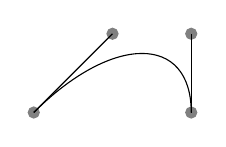
\begin{tikzpicture}
  \filldraw [gray] (0,0) circle (2pt)
  (1,1) circle (2pt)
  (2,1) circle (2pt)
  (2,0) circle (2pt);
  \draw (0,0) .. controls (1,1) and (2,1) .. (2,0);
  \draw (0,0) -- (1,1);
  \draw (2,1) -- (2,0);
\end{tikzpicture}

You can leave out the \keyword{and} (second control point), which causes the first one to be used twice.



\subsection{Circle path}
\label{sec:circle-path}

\begin{lstlisting}
\draw (0,0) circle (10pt);
\end{lstlisting}


\begin{tikzpicture}
  \draw (0,0) circle (10pt);
\end{tikzpicture}



\begin{lstlisting}
\draw (0,0) ellipse (20pt and 10pt);
\end{lstlisting}


\begin{tikzpicture}
  \draw (0,0) ellipse (20pt and 10pt);
\end{tikzpicture}

\subsection{Rectangle path}
\label{sec:rectangle-path}

\begin{lstlisting}
\filldraw [gray] (0,0) circle (2pt);
\filldraw [gray] (0.5,0.5) circle (2pt);
  \draw (0,0) rectangle (0.5,0.5);
\end{lstlisting}


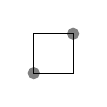
\begin{tikzpicture}
  \filldraw [gray] (0,0) circle (2pt);
  \filldraw [gray] (0.5,0.5) circle (2pt);
  \draw (0,0) rectangle (0.5,0.5);
\end{tikzpicture}

\subsection{Grid path}
\label{sec:grid-path}

\begin{lstlisting}
  \filldraw [gray] (-1.4,-1.4) circle (2pt);
  \filldraw [gray] (1.4,1.4) circle (2pt);

  \draw[step=.5cm,gray,very thin] (-1.4,-1.4) grid (1.4,1.4);
\end{lstlisting}


\begin{tikzpicture}
  \filldraw [gray] (-1.4,-1.4) circle (2pt);
  \filldraw [gray] (1.4,1.4) circle (2pt);

  \draw[step=.5cm,gray,very thin] (-1.4,-1.4) grid (1.4,1.4);
\end{tikzpicture}


\subsection{Arc path}
\label{sec:arc-path}

\begin{lstlisting}
  \filldraw [gray] (0,0) circle (2pt);
  \draw (0mm,0mm) arc (0:30:3cm);
  % (center) arc (angle1:angle2:radius)
  % an arc from angle1 to angle2 on a circle of radius

\end{lstlisting}


\begin{tikzpicture}
  \filldraw [gray] (0,0) circle (2pt);

  \draw (0mm,0mm) arc (0:30:3cm);
  % (center) arc (angle1:angle2:radius)
  % an arc from angle1 to angle2 on a circle of radius
\end{tikzpicture}



\subsection{Clipping a path}
\label{sec:clipping-path}
\begin{lstlisting}
  \draw[step=.5cm,gray,very thin] (-1.4,-1.4) grid (1.4,1.4);
  \draw (-1.5,0) -- (1.5,0);
  \draw (0,-1.5) -- (0,1.5);
  \draw (0,0) circle (1cm);
  \draw (3mm,0mm) arc (0:30:3mm);  

\end{lstlisting}


\begin{tikzpicture}
  \draw[step=.5cm,gray,very thin] (-1.4,-1.4) grid (1.4,1.4);
  \draw (-1.5,0) -- (1.5,0);
  \draw (0,-1.5) -- (0,1.5);
  \draw (0,0) circle (1cm);
  \draw (3mm,0mm) arc (0:30:3mm);  
\end{tikzpicture}

\begin{lstlisting}
  \clip (-0.1,-0.2) rectangle (1.1,0.75);
  \draw[step=.5cm,gray,very thin] (-1.4,-1.4) grid (1.4,1.4);
  \draw (-1.5,0) -- (1.5,0);
  \draw (0,-1.5) -- (0,1.5);
  \draw (0,0) circle (1cm);
  \draw (3mm,0mm) arc (0:30:3mm);  

\end{lstlisting}


\begin{tikzpicture}
  \clip (-0.1,-0.2) rectangle (1.1,0.75);
  \draw[step=.5cm,gray,very thin] (-1.4,-1.4) grid (1.4,1.4);
  \draw (-1.5,0) -- (1.5,0);
  \draw (0,-1.5) -- (0,1.5);
  \draw (0,0) circle (1cm);
  \draw (3mm,0mm) arc (0:30:3mm);  
\end{tikzpicture}

In reality, \keyword{\textbackslash{}draw} is just a shorthand for \keyword{\textbackslash{}path[draw]} and \keyword{\textbackslash{}clip} is a shorthand for \keyword{\textbackslash{}path[clip]} and you could also say \keyword{\textbackslash{}path[draw,clip]}.



\subsection{Filling}
\label{sec:filling}

\begin{lstlisting}
\fill[green!20!white] (0,0) -- (3cm,0cm) arc (0:30:3cm) -- cycle;
\end{lstlisting}


\begin{tikzpicture}
  \fill[green!20!white] (0,0) -- (3cm,0cm) arc (0:30:3cm) -- cycle;
\end{tikzpicture}


The \keyword{--cycle} causes the current path to be closed.


You can also fill and draw a path at the same time using the \keyword{\textbackslash{}filldraw} command.


\subsection{Shading}
\label{sec:shading}

\keyword{\textbackslash{}shade} and \keyword{\textbackslash{}shadedraw} are used for shading and drawing at the same time.

\begin{lstlisting}
  \shade (0,0) rectangle (2,1);
  \shade[top color=yellow,bottom color=black] (3,0) rectangle +(2,1);
  \shade[left color=yellow,right color=black] (6,0) rectangle +(2,1); % relative coordinate
  \shadedraw[inner color=yellow,outer color=black,draw=yellow] (9,0) rectangle +(2,1);
  \shade[ball color=green] (12,.5) circle (.5cm);
\end{lstlisting}


\begin{tikzpicture}
  \shade (0,0) rectangle (2,1);
  \shade[top color=yellow,bottom color=black] (3,0) rectangle +(2,1);
  \shade[left color=yellow,right color=black] (6,0) rectangle +(2,1);
  \shadedraw[inner color=yellow,outer color=black,draw=yellow] (9,0) rectangle +(2,1);
  \shade[ball color=green] (12,.5) circle (.5cm);
\end{tikzpicture}

The default shading is a smooth transition from gray to white. To specify different colors, you can use options.



\subsection{Specifying coordinates}
\label{sec:spec-coord}

\begin{itemize}
\item If you leave out the unites, the default are set to cm and for angle to degree.
\item \keyword{+} means a relative coordinate from the previous specified position and \keyword{++} means a relative coordinate from the previous specified position, making this the new specified position.
\item You can use \keyword{intersection} to specify a coordinate.
\end{itemize}


\begin{lstlisting}
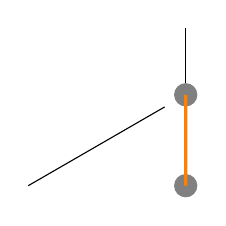
\begin{tikzpicture}[scale=2]
  \draw (1,0) -- (1,1);
  \draw (0,0) -- (30:1cm);
  \filldraw [gray] (1,0) circle (2pt);
  \filldraw [gray] (intersection of 1,0--1,1 and 0,0--30:1cm) circle (2pt);
  \draw[very thick,orange] (1,0) -- (intersection of 1,0--1,1 and 0,0--30:1cm);
\end{tikzpicture}

\end{lstlisting}

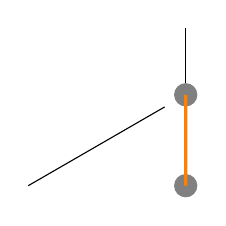
\begin{tikzpicture}[scale=2]
  \draw (1,0) -- (1,1);
  \draw (0,0) -- (30:1cm);
  \filldraw [gray] (1,0) circle (2pt);
  \filldraw [gray] (intersection of 1,0--1,1 and 0,0--30:1cm) circle (2pt);
  \draw[very thick,orange] (1,0) -- (intersection of 1,0--1,1 and 0,0--30:1cm);
\end{tikzpicture}


\subsection{Adding arrow tips}
\label{sec:adding-arrow}


\begin{lstlisting}
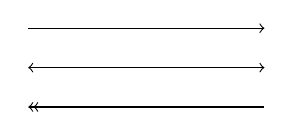
\begin{tikzpicture}
  \draw[->] (-1.5,0) -- (1.5,0);
  \draw[<->] (-1.5,-0.5) -- (1.5,-0.5);
  \draw[<<-] (-1.5,-1) -- (1.5,-1);
\end{tikzpicture}
\end{lstlisting}

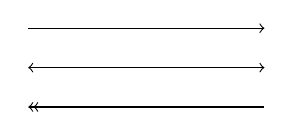
\begin{tikzpicture}
  \draw[->] (-1.5,0) -- (1.5,0);
  \draw[<->] (-1.5,-0.5) -- (1.5,-0.5);
  \draw[<<-] (-1.5,-1) -- (1.5,-1);
\end{tikzpicture}

\begin{lstlisting}
\begin{tikzpicture}[>=stealth]  % >= right arrow tip kind
  \draw[->] (-1.5,0) -- (1.5,0);
\end{tikzpicture}
\end{lstlisting}

\begin{tikzpicture}[>=stealth]  % >= right arrow tip kind
  \draw[->] (-1.5,0) -- (1.5,0);
\end{tikzpicture}



\subsection{Scoping}
\label{sec:scoping}

Scope can let you apply graphic options to a local group.

\begin{lstlisting}
\begin{tikzpicture}[ultra thick]
  \draw (0,0) -- (0,1);
  \begin{scope}[thin]
    \draw (1,0) -- (1,1);
    \draw (2,0) -- (2,1);
  \end{scope}
  \draw (3,0) -- (3,1);
\end{tikzpicture}
\end{lstlisting}

\begin{tikzpicture}[ultra thick]
  \draw (0,0) -- (0,1);
  \begin{scope}[thin]
    \draw (1,0) -- (1,1);
    \draw (2,0) -- (2,1);
  \end{scope}
  \draw (3,0) -- (3,1);
\end{tikzpicture}


\subsection{Transformations}
\label{sec:transformations}

When you specify a coordinate, TikZ applies certain transformations to the given coordinate in order to determine the finally position on the page.

\begin{lstlisting}

\begin{tikzpicture}[even odd rule,rounded corners=2pt,x=10pt,y=10pt]
  % x=10pt set the x unit to 10pt
  \filldraw (0,0)   rectangle (1,1)
  [xshift=5pt,yshift=5pt]   (0,0)   rectangle (1,1)
  [rotate=30]   (-1,-1) rectangle (2,2);

\end{tikzpicture}

\end{lstlisting}


\begin{tikzpicture}[even odd rule,rounded corners=2pt,x=10pt,y=10pt]
  % x=10pt set the x unit to 10pt
  \filldraw (0,0)   rectangle (1,1)
  [xshift=5pt,yshift=5pt]   (0,0)   rectangle (1,1)
  [rotate=30]   (-1,-1) rectangle (2,2);

\end{tikzpicture}

Options to do transformations:
\begin{itemize}
\item \keyword{xshift} and \keyword{yshift}
\item \lstinline|shift={(1,0)}| for shifting to a given point
\item \keyword{rotate} for rotating by a certain angle
\item \keyword{rotate around} for rotating around a given point
\item \keyword{scale} for scaling by a certain factor
\item \keyword{xscale} and \keyword{yscale} (\keyword{xscale=-1} is a flip)
\item \keyword{xslant} and \keyword{yslant} for slanting
\end{itemize}



\subsection{For-loops}
\label{sec:loops}
PGF introduces a command called \keyword{\textbackslash{}foreach}.
The general syntax is
\begin{lstlisting}
\foreach variable in {list of values} command
\end{lstlisting}

\begin{lstlisting}

\begin{tikzpicture}
  \foreach \x in {1,2,...,5,7,9,...,12}
    \foreach \y in {1,...,5}
    {
      \draw (\x,\y) +(-.5,-.5) rectangle ++(.5,.5);
    }
\end{tikzpicture}

\end{lstlisting}


\begin{tikzpicture}
  \foreach \x in {1,2,...,5,7,9,...,12}
    \foreach \y in {1,...,5}
    {
      \draw (\x,\y) +(-.5,-.5) rectangle ++(.5,.5);
    }
\end{tikzpicture}

If you provide two numbers before the \keyword{...}, the \keyword{\textbackslash{}foreach} statement will use their difference for the stepping.




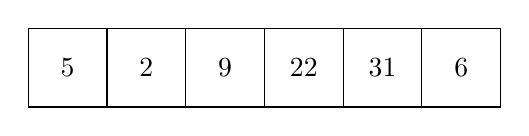
\begin{tikzpicture}
  \foreach \x\y in {0/5,1/2,2/9,3/22,4/31,5/6}
  {
    \node [rectangle,draw,minimum size=1cm] () at (\x ,0) {\y};
  }
\end{tikzpicture}

\begin{lstlisting}

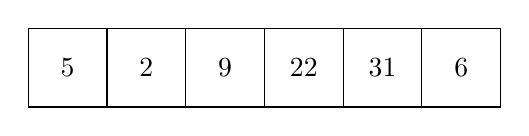
\begin{tikzpicture}
  \foreach \x\y in {0/5,1/2,2/9,3/22,4/31,5/6}
  {
    \node [rectangle,draw,minimum size=1cm] () at (\x ,0) {\y};
  }
\end{tikzpicture}
\end{lstlisting}
\subsection{Adding text}
\label{sec:adding-text}

\begin{lstlisting}
\begin{tikzpicture}
  \draw (0,0) -- node[above=1pt] {above=1pt} (3,0)
  (0,-1) -- node[anchor=north] {anchor=north} (3,-1);
  \draw (0,-3) .. controls (6,-2) and (9,-2) ..
  node[near start,sloped,above] {near start}
  node {midway}
  node[very near end,sloped,below] {very near end} (12,-3);
\end{tikzpicture}
\end{lstlisting}


\begin{tikzpicture}
  \draw (0,0) -- node[above=1pt] {above=1pt} (3,0)
  (0,-1) -- node[anchor=north] {anchor=north} (3,-1);
  \draw (0,-3) .. controls (6,-2) and (9,-2) ..
  node[near start,sloped,above] {near start}
  node {midway}
  node[very near end,sloped,below] {very near end} (12,-3);
\end{tikzpicture}

When TikZ is constructing a path and encounters the keyword \keyword{node} in the middle of a path, it reads a ``node specification''.
The keyword \keyword{node} is typically followed by some options and then some text between curly braces.
This text is put inside a normal TEX box.
All nodes are drawn only after the path has been completely drawn.
You can determine the direction to the position with the \keyword{anchor} option.
And there are simplified writing for the \keyword{anchor} option.
\keyword{below} does the same as \keyword{anchor=south east}.
You can also position labels on curves and, by adding the \keyword{sloped} option, have them rotated such that they match the line’s slope.

\subsection{Load library packages}
\label{sec:load-libr-pack}

\begin{lstlisting}
\usetikzlibrary{arrows,snakes,backgrounds}
\end{lstlisting}




\subsection{Set style}
\label{sec:set-style}

For some commonly used setting, you can set a short name for this setting to save typing and improve clarity.
\begin{lstlisting}
\tikzstyle{place}=[circle,draw=blue!50,fill=blue!20,thick, inner sep=0pt,minimum size=6mm]

\begin{tikzpicture}
  \node [place]  (waiting 1) at (0,2) {};
\end{tikzpicture}
\end{lstlisting}


\subsection{Set color}
\label{sec:set-color}

\begin{lstlisting}
\colorlet{anglecolor}{green!50!black}
\colorlet{sincolor}{red}

\filldraw[fill=green!20,draw=anglecolor] (0,0) -- (3mm,0pt) arc(0:30:3mm);
\end{lstlisting}


\subsection{Local definition}
\label{sec:local-definition}

\begin{lstlisting}
\def\costhirty{0.8660256}
\end{lstlisting}
\subsection{Node}
\label{sec:node}



A node have a \argument{position} and can have a \argument{shape} and \argument{name}.


The \funcword{\textbackslash{}node} command is an abbreviation for \funcword{\textbackslash{}path node}.

\begin{lstlisting}
% shape (circle), style (blue!50,fill=blue!20,thick), size (inner sep=0pt,minimum size=6mm)
\tikzstyle{place}=[circle,draw=blue!50,fill=blue!20,thick,
                   inner sep=0pt,minimum size=6mm]
\tikzstyle{transition}=[rectangle,draw=black!50,fill=black!20,thick,
                        inner sep=0pt,minimum size=4mm]
\begin{tikzpicture}
  % option   name   coordinate  text
  \node[place]      (waiting 1)      at ( 0,2) {};
  \node[place]      (critical 1)     at ( 0,1) {};
  \node[place]      (semaphore)      at ( 0,0) {};
  \node[transition] (leave critical) at ( 1,1) {};
  \node[transition] (enter critical) at (-1,1) {};
\end{tikzpicture}
\end{lstlisting}



% shape (circle), style (blue!50,fill=blue!20,thick), size (inner sep=0pt,minimum size=6mm)
\tikzstyle{place}=[circle,draw=blue!50,fill=blue!20,thick,
                   inner sep=0pt,minimum size=6mm]
\tikzstyle{transition}=[rectangle,draw=black!50,fill=black!20,thick,
                        inner sep=0pt,minimum size=4mm]
\begin{tikzpicture}
  % option   name   coordinate  text
  \node[place]      (waiting 1)      at ( 0,2) {};
  \node[place]      (critical 1)     at ( 0,1) {};
  \node[place]      (semaphore)      at ( 0,0) {};
  \node[transition] (leave critical) at ( 1,1) {};
  \node[transition] (enter critical) at (-1,1) {};
\end{tikzpicture}





We can use relative coordinates and add label to a node.
\begin{lstlisting}
\begin{tikzpicture}
  \tikzstyle{every label}=[red]
  \node[place]   (waiting)      {};                      
  \node[place]   (critical)     [below of=waiting]  {};  
  \node[place]   (semaphore)    [below of=critical,      
                                label=above:$s\le3$] {};   

  \node[transition] (leave critical) [right of=critical] {};
  \node[transition] (enter critical) [left of=critical]  {};
\end{tikzpicture}
\end{lstlisting}


\begin{tikzpicture}
  \tikzstyle{every label}=[red]
  \node[place]   (waiting)      {};                      
  \node[place]   (critical)     [below of=waiting]  {};  
  \node[place]   (semaphore)    [below of=critical,      
                                label=above:$s\le3$] {};   

  \node[transition] (leave critical) [right of=critical] {};
  \node[transition] (enter critical) [left of=critical]  {};
\end{tikzpicture}


We can use \keyword{edge} to draw connection lines.
\begin{lstlisting}
\tikzstyle{pre}=[<-,shorten <=1pt,>=stealth,semithick]
\tikzstyle{post}=[->,shorten >=1pt,>=stealth,semithick]
\begin{tikzpicture}[bend angle=45]
  \node[place]    (waiting)                            {};
  \node[place]    (critical)       [below of=waiting]  {};
  \node[place]    (semaphore)      [below of=critical] {};

  \node[transition] (leave critical) [right of=critical] {}
  edge [pre]                                 (critical)
  edge [post,bend right] node[auto,swap] {2} (waiting)
  edge [pre, bend left]                      (semaphore);
  \node[transition] (enter critical) [left of=critical]  {}
  edge [post]                              (critical) 
  edge [pre, bend left]                    (waiting)
  edge [post,bend right]                   (semaphore);
\end{tikzpicture}
\end{lstlisting}

\tikzstyle{pre}=[<-,shorten <=1pt,>=stealth,semithick]
\tikzstyle{post}=[->,shorten >=1pt,>=stealth,semithick]
\begin{tikzpicture}[bend angle=45]
  \node[place]    (waiting)                            {};
  \node[place]    (critical)       [below of=waiting]  {};
  \node[place]    (semaphore)      [below of=critical] {};

  \node[transition] (leave critical) [right of=critical] {}
  edge [pre]                                 (critical)
  edge [post,bend right] node[auto,swap] {2} (waiting)
  edge [pre, bend left]                      (semaphore);
  \node[transition] (enter critical) [left of=critical]  {}
  edge [post]                              (critical) 
  edge [pre, bend left]                    (waiting)
  edge [post,bend right]                   (semaphore);
\end{tikzpicture}



\subsection{Snake line}
\label{sec:snake-line}
\usetikzlibrary{snakes}
\begin{tikzpicture}
  \draw [->,snake=snake,
         segment amplitude=.4mm,
         segment length=2mm,
         line after snake=1mm] (0,0) -- (3,0);
\end{tikzpicture}


\begin{lstlisting}

\begin{tikzpicture}
  \draw [->,snake=snake,
         segment amplitude=.4mm,
         segment length=2mm,
         line after snake=1mm] (0,0) -- (3,0);
\end{tikzpicture}
\end{lstlisting}
\section{Examples}
\label{sec:examples}

\subsection{A picture for Karl’s students}
\label{sec:pict-karls-stud}

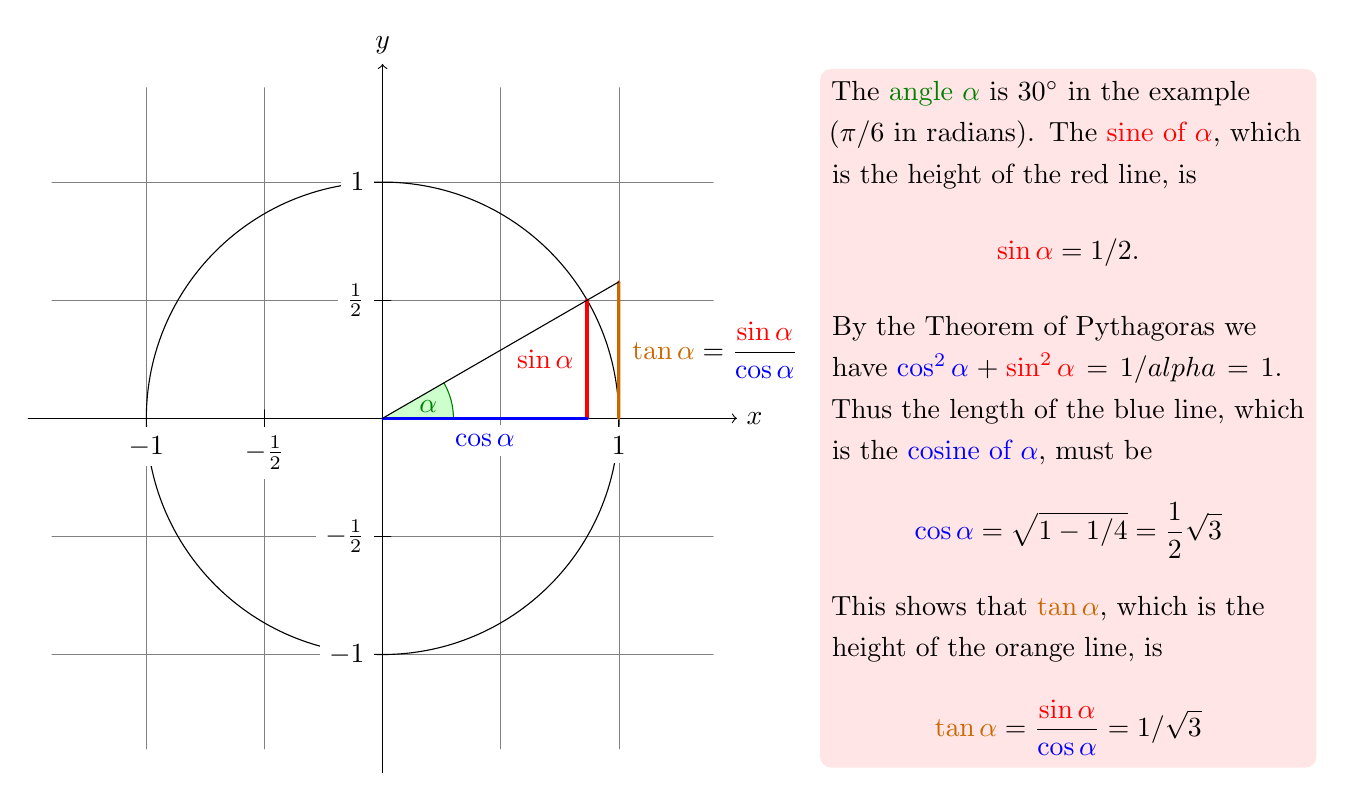
\begin{tikzpicture}[scale=3,cap=round]
  % Local definitions
  \def\costhirty{0.8660256}
  % Colors
  \colorlet{anglecolor}{green!50!black}
  \colorlet{sincolor}{red}
  \colorlet{tancolor}{orange!80!black}
  \colorlet{coscolor}{blue}
  % Styles
  \tikzstyle{axes}=[]
  \tikzstyle{important line}=[very thick]
  \tikzstyle{information text}=[rounded corners,fill=red!10,inner sep=1ex]
  % The graphic
  \draw[style=help lines,step=0.5cm] (-1.4,-1.4) grid (1.4,1.4);
  \draw (0,0) circle (1cm);
  \begin{scope}[style=axes]
    \draw[->] (-1.5,0) -- (1.5,0) node[right] {$x$} coordinate(x axis);
    \draw[->] (0,-1.5) -- (0,1.5) node[above] {$y$} coordinate(y axis);
    \foreach \x/\xtext in {-1, -.5/-\frac{1}{2}, 1}
    \draw[xshift=\x cm] (0pt,1pt) -- (0pt,-1pt) node[below,fill=white] {$\xtext$};
    \foreach \y/\ytext in {-1, -.5/-\frac{1}{2}, .5/\frac{1}{2}, 1}
    \draw[yshift=\y cm] (1pt,0pt) -- (-1pt,0pt) node[left,fill=white] {$\ytext$};
  \end{scope}
  \filldraw[fill=green!20,draw=anglecolor] (0,0) -- (3mm,0pt) arc(0:30:3mm);
  \draw (15:2mm) node[anglecolor] {$\alpha$};
  \draw[style=important line,sincolor]
  (30:1cm) -- node[left=1pt,fill=white] {$\sin \alpha$} (30:1cm |- x axis);
  \draw[style=important line,coscolor]
  (30:1cm |- x axis) -- node[below=2pt,fill=white] {$\cos \alpha$} (0,0);
  \draw[style=important line,tancolor] (1,0) -- node[right=1pt,fill=white] {
    $\displaystyle \tan \alpha \color{black}=
    \frac{{\color{sincolor}\sin \alpha}}{\color{coscolor}\cos \alpha}$}
  (intersection of 0,0--30:1cm and 1,0--1,1) coordinate (t);
  \draw (0,0) -- (t);
  \draw[xshift=1.85cm]
  node[right,text width=6cm,style=information text]
  {
    The {\color{anglecolor} angle $\alpha$} is $30^\circ$ in the
      example ($\pi/6$ in radians). The {\color{sincolor}sine of
        $\alpha$}, which is the height of the red line, is
      \[
      {\color{sincolor} \sin \alpha} = 1/2.
      \]

      By the Theorem of Pythagoras we have ${\color{coscolor}\cos ^2 \alpha}+{\color{sincolor} \sin^{2} \alpha} = 1/alpha=1$.
      Thus the length of the blue line, which is the {\color{coscolor} cosine of $\alpha$}, must be
    $$
    {\color{coscolor}\cos \alpha}=\sqrt{1-1 / 4}=\frac{1}{2} \sqrt{3}
    $$
    This shows that {\color{tancolor}$\tan \alpha$}, which is the height of the orange line, is
    $$
    {\color{tancolor}\tan \alpha}=\frac{\color{sincolor}\sin \alpha}{\color{coscolor}\cos \alpha}=1 / \sqrt{3}
    $$
  };
\end{tikzpicture}

\begin{lstlisting}
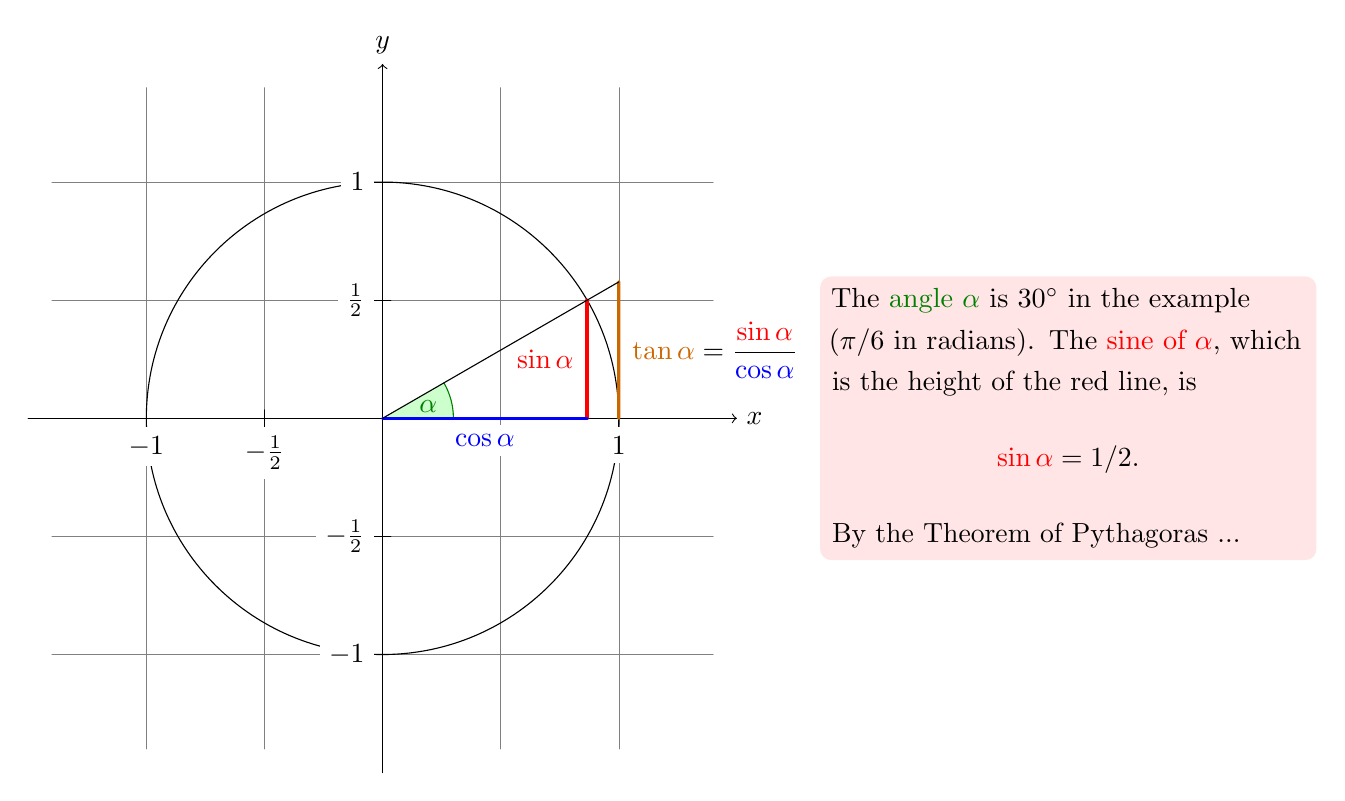
\begin{tikzpicture}[scale=3,cap=round]
% Local definitions
  \def\costhirty{0.8660256}
% Colors
  \colorlet{anglecolor}{green!50!black}
  \colorlet{sincolor}{red}
  \colorlet{tancolor}{orange!80!black}
  \colorlet{coscolor}{blue}
% Styles
  \tikzstyle{axes}=[]
  \tikzstyle{important line}=[very thick]
  \tikzstyle{information text}=[rounded corners,fill=red!10,inner sep=1ex]
% The graphic
  \draw[style=help lines,step=0.5cm] (-1.4,-1.4) grid (1.4,1.4);
  \draw (0,0) circle (1cm);
  \begin{scope}[style=axes]
    \draw[->] (-1.5,0) -- (1.5,0) node[right] {$x$} coordinate(x axis);
    \draw[->] (0,-1.5) -- (0,1.5) node[above] {$y$} coordinate(y axis);
    \foreach \x/\xtext in {-1, -.5/-\frac{1}{2}, 1}
      \draw[xshift=\x cm] (0pt,1pt) -- (0pt,-1pt) node[below,fill=white] {$\xtext$};
    \foreach \y/\ytext in {-1, -.5/-\frac{1}{2}, .5/\frac{1}{2}, 1}
      \draw[yshift=\y cm] (1pt,0pt) -- (-1pt,0pt) node[left,fill=white] {$\ytext$};
\end{scope}
  \filldraw[fill=green!20,draw=anglecolor] (0,0) -- (3mm,0pt) arc(0:30:3mm);
  \draw (15:2mm) node[anglecolor] {$\alpha$};
  \draw[style=important line,sincolor]
    (30:1cm) -- node[left=1pt,fill=white] {$\sin \alpha$} (30:1cm |- x axis);
  \draw[style=important line,coscolor]
    (30:1cm |- x axis) -- node[below=2pt,fill=white] {$\cos \alpha$} (0,0);
  \draw[style=important line,tancolor] (1,0) -- node[right=1pt,fill=white] {
    $\displaystyle \tan \alpha \color{black}=
    \frac{{\color{sincolor}\sin \alpha}}{\color{coscolor}\cos \alpha}$}
    (intersection of 0,0--30:1cm and 1,0--1,1) coordinate (t);
  \draw (0,0) -- (t);
  \draw[xshift=1.85cm]
    node[right,text width=6cm,style=information text]
    {
      The {\color{anglecolor} angle $\alpha$} is $30^\circ$ in the
      example ($\pi/6$ in radians). The {\color{sincolor}sine of
        $\alpha$}, which is the height of the red line, is
      \[
      {\color{sincolor} \sin \alpha} = 1/2.
      \]
      By the Theorem of Pythagoras ...
    };
\end{tikzpicture}
\end{lstlisting}



\subsection{A Petri-Net for Hagen}
\label{sec:petri-net-hagen}

\usetikzlibrary{arrows,snakes,backgrounds}

\tikzstyle{place}=[circle,draw=blue!50,fill=blue!20,thick,inner sep=0pt,minimum size=6mm]
\tikzstyle{transition}=[rectangle,draw=black!50,fill=black!20,thick,inner sep=0pt,minimum size=4mm]

\tikzstyle{pre}=[<-,shorten <=1pt,>=stealth,semithick]
\tikzstyle{post}=[->,shorten >=1pt,>=stealth,semithick]

\tikzstyle{every place}=[minimum size=6cm,thick,draw=blue!75,fill=blue!20]
\tikzstyle{every transition}=[thick,draw=black!75,fill=black!20]
\tikzstyle{red place}=[place,draw=red!75,fill=red!20]
\tikzstyle{every label}=[red]


\begin{tikzpicture}[node distance=1.3cm,>=stealth,bend angle=45,auto]
  \node [place] (w1)  {};
  \node [place] (c1) [below of=w1] {};
  \node [place] (s) [below of=c1,label=above:\(s\le 3\)] {};
  \node [place] (c2) [below of=s] {};
  \node [place] (w2) [below of=c2] {};

  \node [transition] (e1) [left of=c1] {}
  edge [pre,bend left] (w1)
  edge [post,bend right] (s)
  edge [post] (c1);
  \node [transition] (e2) [left of=c2] {}
  edge [pre, bend right] (w2)
  edge [pre, bend left] (s)
  edge [post] (c2);
  \node [transition] (l1) [right of=c1] {}
  edge [pre] (c1)
  edge [pre,bend left] (s)
  edge [post,bend right] node [swap] {2} (w1);
  \node [transition] (l2) [right of=c2] {}
  edge [pre] (c2)
  edge [pre,bend right] (s)
  edge [post,bend left] node {2} (w2);

  \begin{scope}[xshift=6cm]
    \node [place] (w1') {};
    \node [place] (c1') [below of=w1'] {};
    \node [red place] (s1') [below of=c1',xshift=-0.5cm] [label=left:\(s\)] {};
    \node [red place] (s2') [below of=c1',xshift=0.5cm] [label=right:\(\bar s\)] {};
    \node [place] (c2') [below of=s1',xshift=.5cm] {};
    \node [place] (w2') [below of=c2'] {};

    \node [transition] (e1') [left of=c1'] {}
    edge [pre,bend left] (w1')
    edge [post] (s1')
    edge [pre] (s2')
    edge [post] (c1');
    \node [transition] (e2') [left of=c2'] {}
    edge [pre,bend right] (w2')
    edge [post] (s1')
    edge [pre] (s2')
    edge [post] (c2');
    \node [transition] (l1') [right of=c1'] {}
    edge [pre] (c1')
    edge [pre] (s1')
    edge [post] (s2')
    edge [post,bend right] node [swap]  {2} (w1');
    \node [transition] (l2') [right of=c2'] {}
    edge [pre] (c2')
    edge [pre] (s1')
    edge [post] (s2')
    edge [post,bend left] node {2} (w2');
  \end{scope}

  \draw [-to,thick,snake=snake,segment amplitude=.4mm,segment length=2mm,line after snake=1mm]
    ([xshift=5mm]s -| l1) -- ([xshift=-5mm]s1' -| e1')
    node [above=1mm,midway,text width=3cm,text centered]
      {replacement of the \textcolor{red}{capacity} by \textcolor{red}{two places}};
  \begin{pgfonlayer}{background}
    \filldraw [line width=4mm,join=round,black!10]
      (w1.north  -| l1.east)  rectangle (w2.south  -| e1.west)
      (w1'.north -| l1'.east) rectangle (w2'.south -| e1'.west);
  \end{pgfonlayer}
\end{tikzpicture}


\begin{lstlisting}
\usetikzlibrary{arrows,snakes,backgrounds}

\tikzstyle{place}=[circle,draw=blue!50,fill=blue!20,thick,inner sep=0pt,minimum size=6mm]
\tikzstyle{transition}=[rectangle,draw=black!50,fill=black!20,thick,inner sep=0pt,minimum size=4mm]

\tikzstyle{pre}=[<-,shorten <=1pt,>=stealth,semithick]
\tikzstyle{post}=[->,shorten >=1pt,>=stealth,semithick]

\tikzstyle{every place}=[minimum size=6cm,thick,draw=blue!75,fill=blue!20]
\tikzstyle{every transition}=[thick,draw=black!75,fill=black!20]
\tikzstyle{red place}=[place,draw=red!75,fill=red!20]
\tikzstyle{every label}=[red]


\begin{tikzpicture}[node distance=1.3cm,>=stealth,bend angle=45,auto]
  \node [place] (w1)  {};
  \node [place] (c1) [below of=w1] {};
  \node [place] (s) [below of=c1,label=above:\(s\le 3\)] {};
  \node [place] (c2) [below of=s] {};
  \node [place] (w2) [below of=c2] {};

  \node [transition] (e1) [left of=c1] {}
  edge [pre,bend left] (w1)
  edge [post,bend right] (s)
  edge [post] (c1);
  \node [transition] (e2) [left of=c2] {}
  edge [pre, bend right] (w2)
  edge [pre, bend left] (s)
  edge [post] (c2);
  \node [transition] (l1) [right of=c1] {}
  edge [pre] (c1)
  edge [pre,bend left] (s)
  edge [post,bend right] node [swap] {2} (w1);
  \node [transition] (l2) [right of=c2] {}
  edge [pre] (c2)
  edge [pre,bend right] (s)
  edge [post,bend left] node {2} (w2);

  \begin{scope}[xshift=6cm]
    \node [place] (w1') {};
    \node [place] (c1') [below of=w1'] {};
    \node [red place] (s1') [below of=c1',xshift=-0.5cm] [label=left:\(s\)] {};
    \node [red place] (s2') [below of=c1',xshift=0.5cm] [label=right:\(\bar s\)] {};
    \node [place] (c2') [below of=s1',xshift=.5cm] {};
    \node [place] (w2') [below of=c2'] {};

    \node [transition] (e1') [left of=c1'] {}
    edge [pre,bend left] (w1')
    edge [post] (s1')
    edge [pre] (s2')
    edge [post] (c1');
    \node [transition] (e2') [left of=c2'] {}
    edge [pre,bend right] (w2')
    edge [post] (s1')
    edge [pre] (s2')
    edge [post] (c2');
    \node [transition] (l1') [right of=c1'] {}
    edge [pre] (c1')
    edge [pre] (s1')
    edge [post] (s2')
    edge [post,bend right] node [swap]  {2} (w1');
    \node [transition] (l2') [right of=c2'] {}
    edge [pre] (c2')
    edge [pre] (s1')
    edge [post] (s2')
    edge [post,bend left] node {2} (w2');
  \end{scope}

  \draw [-to,thick,snake=snake,segment amplitude=.4mm,segment length=2mm,line after snake=1mm]
    ([xshift=5mm]s -| l1) -- ([xshift=-5mm]s1' -| e1')
    node [above=1mm,midway,text width=3cm,text centered]
      {replacement of the \textcolor{red}{capacity} by \textcolor{red}{two places}};
  \begin{pgfonlayer}{background}
    \filldraw [line width=4mm,join=round,black!10]
      (w1.north  -| l1.east)  rectangle (w2.south  -| e1.west)
      (w1'.north -| l1'.east) rectangle (w2'.south -| e1'.west);
  \end{pgfonlayer}
\end{tikzpicture}

\end{lstlisting}
%%% Local Variables:
%%% mode: latex
%%% TeX-master: "latex"
%%% End:


\chapter{Reference}
\label{cha:reference}

\begin{lstlisting}
% \usepackage{amssymb}
\checkmark{}
\end{lstlisting}
\checkmark{}
%%% Local Variables:
%%% mode: latex
%%% TeX-master: "latex"
%%% End:



% Pages are numbered with Arabic numbers.
% Chapters generate a table of contents entry but don't get a number.
\backmatter
\nocite{*}
\bibliographystyle{alpha}
\bibliography{tex}

\clearpage{}
% just setting an anchor like \hypertarget{}{}
% fix the problem that anchor point to the previous section
\phantomsection                 
\printindex{}
\end{document}

%%% Local Variables:
%%% mode: latex
%%% TeX-master: t
%%% End:

